\begin{name}
	{\tenchude}{\tendethi}{LỚP TOÁN THẦY PHÁT}{\thoigian}
\end{name}
%\setcounter{ex}{0}
\Opensolutionfile{ans}[ans/ans-2-TT-16-PhuDuc-ThaiBinh-23]

\begin{ex}%[Lương Như Quỳnh]%[12-EX-6-2023]%[2D2B6-2]
Tập nghiệm của bất phương trình $2^{x+1}\le 4$ là
\choice
{\True $(-\infty ;1]$}
{$(1;+\infty)$}
{$[1;+\infty)$}
{$(-\infty ;1)$}
\loigiai{Ta có $$2^{x+1}\le 4\Leftrightarrow2^{x+1}\le 2^2\Leftrightarrow x+1 \le 2 \Leftrightarrow x\le 1.$$
Vậy bất phương trình có tập nghiệm là $(-\infty ;1]$.}
\end{ex}

\begin{ex}%[Lương Như Quỳnh]%[12-EX-6-2023]%[2D2B5-3]
Tích tất cả các nghiệm của phương trình $\log_2^2x-3\log_2x+2=0$ bằng
\choice
{\True $8$}
{$6$}
{$16$}
{$2$}
\loigiai{Ta có $$\log_2^2x-3\log_2x+2=0\Leftrightarrow \hoac{&\log_2x=1\\&\log_2x=2}\Leftrightarrow\hoac{&x=2\\&x=4.}$$ 
Vậy tích các nghiệm của phương trình đã cho bằng $8$.}
\end{ex}

\begin{ex}%[Lương Như Quỳnh]%[12-EX-6-2023]%[2D3B1-1]
Cho $\displaystyle\int \dfrac{1}{x{\ln^2}x}\mathrm{\,d}x=F(x)+C$. Khẳng định nào dưới đây đúng?
\choice
{$F'(x)=\dfrac{-1}{\ln\text{x}}$}
{$F'(x)=\dfrac{-1}{\ln\text{x}}+C$}
{\True $F'(x)=\dfrac{1}{x{\ln^2}x}$}
{$F'(x)=-\dfrac{1}{\ln^2x}$}
\loigiai{
Lấy đạo hàm hai vế theo biến $x$ của đẳng thức đã cho, ta được $$\left(\displaystyle\int \dfrac{1}{x{\ln^2}x}\mathrm{\,d}x\right)'=\left(F(x)+C\right)'\Leftrightarrow \dfrac{1}{x{\ln^2}x}=F'(x).$$
Vậy  $F'(x)=\dfrac{1}{x{\ln^2}x}$.
}
\end{ex}

\begin{ex}%[Lương Như Quỳnh]%[12-EX-6-2023]%[2H3Y3-2]
Trong không gian với hệ trục tọa độ $Oxyz$, cho đường thẳng $d\colon \dfrac{x-1}{3}=\dfrac{y+2}{-4}=\dfrac{z-3}{-5}$. Hỏi $d$ đi qua điểm nào trong các điểm sau đây?
\choice
{$C(-3;4;5)$}
{$D(3;-4;-5)$}
{$B(-1;2;-3)$}
{\True $A(1;-2;3)$}
\loigiai{Ta thấy tọa độ của điểm $A(1;-2;3)$ thỏa mãn phương trình của $d$ nên $d$ đi qua điểm $A$.}
\end{ex}

\begin{ex}%[Lương Như Quỳnh]%[12-EX-6-2023]%[2H1Y3-2]
\immini{Cho khối chóp $S.ABC$ có đáy là tam giác vuông cân tại $A$, $AB=2$, $SA$ vuông góc với đáy và $SA=3$. Thể tích khối chóp đã cho bằng
\choice
{$12$}
{\True $2$}
{$6$}
{$4$}}
{
\begin{tikzpicture}[>=stealth,line join=round,line cap=round,font=\footnotesize,scale=.6]
\path 
(0,0) coordinate (A)
(-1.5,-1.5) coordinate (B)
(5,0) coordinate (C)
($(A)+(90:4)$) coordinate (S)
;
\draw (S)--(B)--(C)--cycle;
\draw[dashed] (A)--(B) (S)--(A)--(C) ;
\foreach\p/\g in {S/90, A/180, B/-70, C/0}
\draw[fill=black] (\p) circle (1pt) node[shift=(\g:3mm)] {$\p$};
\tkzMarkRightAngle (B,A,C)
\end{tikzpicture}
}
\loigiai{
Thể tích của khối chóp đã cho là $$V=\dfrac{1}{3}\cdot S_{ABC}\cdot SA=\dfrac{1}{3}\cdot\dfrac{1}{2}\cdot 2^2\cdot3=2. $$
}
\end{ex}

\begin{ex}%[Lương Như Quỳnh]%[12-EX-6-2023]%[2H3Y1-3]
Trong KG $Oxyz$, cho mặt cầu $(S)\colon x^2+y^2+z^2-2x+2y-4z-2=0$. Tính bán kính $r$ của mặt cầu.
\choice
{\True $r=2\sqrt{2}$}
{$r=\sqrt{26}$}
{$r=4$}
{$r=\sqrt{2}$}
\loigiai{
Ta có  $$(S)\colon {x^2}+y^2+z^2-2x+2y-4z-2=0\Leftrightarrow (x-1)^2+(y+1)^2+(z-2)^2=8.$$
Vậy bán kính của mặt cầu là $r=2\sqrt{2}$.}
\end{ex}

\begin{ex}%[Lương Như Quỳnh]%[12-EX-6-2023]%[1D2Y2-1]
Cho một tổ có $15$ thành viên. Số cách chọn ra $2$ người lần lượt làm tổ trưởng và tổ phó là
\choice
{$225$}
{$30$}
{\True $210$}
{$105$}
\loigiai{
Số cách chọn ra $2$ người lần lượt làm tổ trưởng và tổ phó là một chỉnh hợp chập $2$ của $15$ phần tử.\\
Vậy có $\mathrm{A}_{15}^2$ cách chọn.
}
\end{ex}

\begin{ex}%[Lương Như Quỳnh]%[12-EX-6-2023]%[2H3Y1-1]
Trong KG $Oxyz$, cho điểm $A(1;2;3)$. Điểm đối xứng với $A$ qua mặt phẳng $(Oyz)$ có tọa độ là
\choice
{$(1;-2;3)$}
{$(1;2;-3)$}
{$(-1;-2;-3)$}
{\True $(-1;2;3)$}
\loigiai{
Điểm đối xứng với $A(1;2;3)$ qua mặt phẳng $(Oyz)$ có tọa độ là $(-1;2;3)$.
}
\end{ex}

\begin{ex}%[Lương Như Quỳnh]%[12-EX-6-2023]%[2H3Y2-2]
Trong KG $Oxyz$, mặt phẳng $(P)\colon x-2z+3=0$ có một véc-tơ pháp tuyến là 
\choice
{\True $\overrightarrow{n}_{1}=(1;0;-2)$}
{$\overrightarrow{n}_{4}=(1;-2;3)$}
{$\overrightarrow{n}_{3}=(1;-2;0)$}
{$\overrightarrow{n}_{2}=(-1;2;-3)$}
\loigiai{
Mặt phẳng $(P)\colon x-2z+3=0$ có một véc-tơ pháp tuyến là $\overrightarrow{n}_{1}=(1;0;-2)$.}
\end{ex}

\begin{ex}%[Lương Như Quỳnh]%[12-EX-6-2023]%[2D2Y4-2]
Đạo hàm của hàm số $y=\pi^x$ là 
\choice
{\True $y'=\pi^x\ln\pi $}
{$y'=x\cdot \pi^{x-1}$}
{$y'=\dfrac{\pi^x}{\ln\pi}$}
{$y'=\dfrac{\pi^{x+1}}{x+1}$}
\loigiai{
Hàm số $y=\pi^x$ là hàm số mũ cơ số $\pi$ nên có đạo hàm là $y'=\pi^x\ln\pi$.
}
\end{ex}

\begin{ex}%[Lương Như Quỳnh]%[12-EX-6-2023]%[2H3Y3-2]
Trong KG $Oxyz$, cho hai điểm $M(1;-1;-1)$ và $N(5;5;1)$. Đường thẳng $MN$ có phương trình là 
\choice
{$\heva{&x=5+2t\\&y=5+3t\\&z=-1+t}$}
{$\heva{&x=5+t\\&y=5+2t\\&z=1+3t}$}
{\True $\heva{&x=3+2t\\&y=2+3t\\&z=t}$}
{$\heva{&x=1+2t\\&y=-1+t\\&z=-1+3t}$}
\loigiai{Ta có $\overrightarrow{MN}=(4;6;2)=2\overrightarrow{u}$ với $\overrightarrow{u}=(2;3;1)$ nên loại các phương trình $\heva{&x=5+2t\\&y=5+3t\\&z=-1+t}$, $\heva{&x=5+t\\&y=5+2t\\&z=1+3t.}$\\
Thay tọa độ của $M(1;-1;-1)$ vào phương trình $\heva{&x=3+2t\\&y=2+3t\\&z=t}$ ta thấy thỏa mãn nên đây là PTTS của đường thẳng $MN$.}
\end{ex}

\begin{ex}%[Lương Như Quỳnh]%[12-EX-6-2023]%[2D1Y5-1]
	\immini{
Cho hàm số $y=\dfrac{ax+b}{cx+d}$ có đồ thị là đường cong trong hình vẽ. Tọa độ giao điểm của đồ thị hàm số đã cho và trục tung là
\choice
{\True $(0;-2)$}
{$(2;0)$}
{$(-2;0)$}
{$(0;2)$}}{
\begin{tikzpicture}[line join=round, line cap=round,>=stealth,scale=0.6]
\tikzset{every node/.style={scale=0.9}}
\draw[->] (-6.6,0)--(4.6,0) node[below left] {$x$};
\draw[->] (0,-3.6)--(0,5.1) node[below left] {$y$};
\draw (0,0) node [below left] {$O$};
\foreach \x in {2}
\draw[thin] (\x,1pt)--(\x,-1pt) node [below] {$\x$};
\foreach \y in {1}
\draw[thin] (1pt,\y)--(-1pt,\y) node [above left] {$\y$};
\foreach \y in {-2}
\draw[thin] (1pt,\y)--(-1pt,\y) node [left] {$\y$};
\draw (-1,-3.5)--(-1,5);	
\begin{scope}
\clip (-6.5,-3.5) rectangle (4.5,5);
			\draw[samples=200,domain=-4:-1.01,smooth,variable=\x] plot (\x,{(1*(\x)+-2)/(1*(\x)+1)});	\draw[samples=200,domain=-0.99:3,smooth,variable=\x] plot (\x,{(1*(\x)+-2)/(1*(\x)+1)});	\draw[samples=200,domain=-6.5:-1.01,smooth,variable=\x] plot (\x,{(1*(\x)+-2)/(1*(\x)+1)});		\draw[samples=200,domain=-0.99:4.5,smooth,variable=\x] plot (\x,{(1*(\x)+-2)/(1*(\x)+1)});
\draw(-6.5,1/1)--(4.5,1/1);
\end{scope}
\fill (-1,0) circle(1pt) node[below left]{$-1$}(0,0) circle(1pt);
\end{tikzpicture}
}
\loigiai{
Từ đồ thị ta thấy tọa độ giao điểm của đồ thị hàm số và trục tung là $(0;-2)$.
}
\end{ex}

\begin{ex}%[Lương Như Quỳnh]%[12-EX-6-2023]%[2D1Y2-2]
	\immini{
Cho hàm số $y=f(x)$ xác định và liên tục trên đoạn có $[-2;2]$ và có đồ thị là đường cong trong hình vẽ. Giá trị cực tiểu của hàm số $y=f(x)$ là
\choice
{$-4$}
{\True $-2$}
{$(1;-2)$}
{$x=1$}}{
\begin{tikzpicture}[>=stealth,line join=round,line cap=round,font=\footnotesize,yscale=0.6]
		\draw[->] (-3.1,0)--(3.1,0) node[below left] {$x$};
		\draw[->] (0,-5.1)--(0,5.1) node[below left] {$y$};
		\draw (0,0) node [below left] {$O$};
		\draw[dashed](-2,0)--(-2,-4)--(0,-4);
		\draw[dashed](-0.91,0)--(-0.91,2.03)--(0,2);
		\draw[dashed](0.91,0)--(0.91,-2.03)--(0,-2);
		\draw[dashed](2,0)--(2,4)--(0,4);
		\fill (-2,0) circle(1pt) node[above]{$-2$}
		(2,0) circle(1pt) node[below]{$2$}
		(0,4) circle(1pt) node[left]{$4$}
		(0,-2) circle(1pt) node[left]{$-2$}
		(0,2) circle(1pt) node[right]{$2$}
		(0,-4) circle(1pt) node[right]{$-4$}
		(-0.91,0) circle(1pt) node[below]{$-1$}
		(0.91,0) circle(1pt) node[above]{$1$};
		\begin{scope}
		\clip (-3,-5) rectangle (3,5);
			\draw[samples=200,domain=-2.2:2.2,smooth,variable=\x] plot (\x,{(4/3)*((\x)^3)+0*((\x)^2)-(10/3)*(\x)+0});
		\end{scope}
	\end{tikzpicture}}
\loigiai{Từ đồ thị ta thấy, hàm số đạt cực tiểu tại điểm $x=1$ và giá trị cực tiểu là $y=-2$.}
\end{ex}

\begin{ex}%[Lương Như Quỳnh]%[12-EX-6-2023]%[2D1B5-4]
	\immini{
Cho hàm số bậc ba $y=f(x)$ có đồ thị là đường cong trong hình vẽ. Có bao nhiêu giá trị nguyên của tham số $m$ để phương trình $f(x)=m$ có ba nghiệm thực phân biệt?
\choice
{$2$}
{$5$}
{\True $3$}
{$4$}}{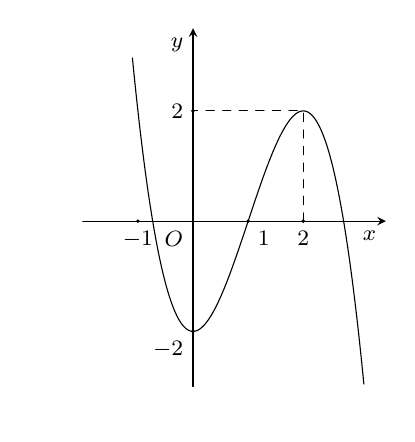
\begin{tikzpicture}[>=stealth,line join=round,line cap=round,font=\footnotesize,scale=0.7]
	\draw[->] (-2,0)--(3.5,0) node[below left] {$x$};
	\draw[->] (0,-3)--(0,3.5) node[below left] {$y$};
	\draw (0,0) node [below left] {$O$};
	\draw[dashed](2,0)--(2,2)--(0,2);
	\fill 
	(2,0) circle(1pt) node[below]{$2$}
	(0,-2) circle(1pt) node[below left]{$-2$}
	(0,2) circle(1pt) node[left]{$2$}
	(-1,0) circle(1pt) node[below]{$-1$}
	(1,0) circle(1pt) node[below right]{$1$};
	\begin{scope}
	\clip (-3,-3.5) rectangle (3.5,3.5);
		\draw[samples=200,domain=-1.1:3.1,smooth,variable=\x] plot (\x,{(-1)*((\x)^3)+3*((\x)^2)-2});
	\end{scope}
\end{tikzpicture}}
\loigiai{Từ đồ thị ta thấy phương trình $f(x)=m$ có ba nghiệm thực phân biệt khi và chỉ khi $-2<m<2$.\\
Mà $ m $ nguyên nên $ m\in \{-1,0,1\} $. Vậy có $ 3 $ giá trị của $ m $ thỏa mãn. }
\end{ex}

\begin{ex}%[Lương Như Quỳnh]%[12-EX-6-2023]%[2D3Y3-1]
Cho hàm số $y=f(x)$ liên tục trên đoạn $[a;b]$. Diện tích hình phẳng giới hạn bởi đồ thị hàm số $y=f(x)$, trục hoành và hai đường thẳng $x=a$; $x=b$ $(a<b)$ là
\choice
{$S=\displaystyle\int\limits_b^a{\left| f(x)\right|}\mathrm{\,d}x$}
{$S=\displaystyle\int\limits_a^b{f(x)}\mathrm{\,d}x$}
{\True $S=\displaystyle\int\limits_a^b{\left| f(x)\right|}\mathrm{\,d}x$}
{$S=\displaystyle\int\limits_b^a{f(x)}\mathrm{\,d}x$}
\loigiai{ Diện tích hình phẳng giới hạn bởi đồ thị hàm số $y=f(x)$, trục hoành và hai đường thẳng $x=a$; $x=b$ $(a<b)$ là $$S=\displaystyle\int\limits_a^b{\left| f(x)\right|}\mathrm{\,d}x.$$}
\end{ex}

\begin{ex}%[Lương Như Quỳnh]%[12-EX-6-2023]%[2D2Y4-2]
Trên tập $\mathbb{R}\setminus\left\{ 0\right\}$, đạo hàm của hàm số $y=\log_3|x|$ là 
\choice
{\True $y'=\dfrac{1}{\left| x\right|\ln 3}$}
{$y'=\dfrac{1}{x\ln 3}$}
{$y'=\dfrac{\ln 3}{x}$}
{$y'=-\dfrac{1}{x\ln 3}$}
\loigiai{
Trên tập $\mathbb{R}\setminus\left\{ 0\right\}$, đạo hàm của hàm số $y=\log_3|x|$ là $y'=\dfrac{1}{\left| x\right|\ln 3}$.}
\end{ex}
\begin{ex}%[Lương Như Quỳnh]%[12-EX-6-2023]%[2D1Y1-2]
	\immini{
Cho đồ thị hàm số $y=f(x)$ có đồ thị như hình vẽ. Hàm số $y=f(x)$ đồng biến trên khoảng nào dưới đây?
\choice
{$(-2;2)$}
{$(-\,\infty ;0)$}
{\True $(0;2)$}
{$(2;+\infty)$}}{\begin{tikzpicture}[>=stealth,line join=round,line cap=round,font=\footnotesize,scale=0.8]
	\draw[->] (-2,0)--(3.6,0) node[below left] {$x$};
	\draw[->] (0,-3)--(0,3.5) node[below left] {$y$};
	\draw (0,0) node [below left] {$O$};
	\draw[dashed](2,0)--(2,2)--(0,2);
	\fill 
	(2,0) circle(1pt) node[below]{$2$}
	(0,-2) circle(1pt) node[below left]{$-2$}
	(0,2) circle(1pt) node[left]{$2$}
	(-1,0) circle(1pt) node[below]{$-1$}
	(1,0) circle(1pt) node[below right]{$1$};
	\begin{scope}
	\clip (-3,-3) rectangle (3,3.5);
	\draw[samples=200,domain=-1.1:3.4,smooth,variable=\x] plot (\x,{(-1)*((\x)^3)+3*((\x)^2)-2});
	\end{scope}
\end{tikzpicture}}
\loigiai{Từ đồ thị ta thấy hàm số đã cho đồng biến trên khoảng $(0;2)$.}
\end{ex}

\begin{ex}%[Lương Như Quỳnh]%[12-EX-6-2023]%[2D1Y5-1]
	\immini{
Đồ thị của hàm số nào dưới đây có dạng như đường cong trong hình vẽ?
\choice
{$y=\dfrac{x+3}{x-1}$}
{\True $y=\dfrac{x-3}{x-1}$}
{$y=x^2-4x+1$}
{$y=x^3-3x-5$}}{\begin{tikzpicture}[line join=round, line cap=round,>=stealth,scale=0.5]
	\draw[->] (-6.6,0)--(4.6,0) node[below left] {$x$};
	\draw[->] (-2,-3.6)--(-2,5.1) node[below left] {$y$};
	\draw (-2,0) node [below left] {$O$};

	\draw (-1,-3.5)--(-1,5);	
	\begin{scope}
		\clip (-6.5,-3.5) rectangle (4.5,5);
		\draw[samples=200,domain=-4:-1.01,smooth,variable=\x] plot (\x,{(1*(\x)+-2)/(1*(\x)+1)});
		\draw[samples=200,domain=-0.99:3,smooth,variable=\x] plot (\x,{(1*(\x)+-2)/(1*(\x)+1)});
		\draw[samples=200,domain=-6.5:-1.01,smooth,variable=\x] plot (\x,{(1*(\x)+-2)/(1*(\x)+1)});
		\draw[samples=200,domain=-0.99:4.5,smooth,variable=\x] plot (\x,{(1*(\x)+-2)/(1*(\x)+1)});
		\draw(-6.5,1/1)--(4.5,1/1);
	\end{scope}
\end{tikzpicture}}
\loigiai{
Đồ thị hàm số có đường tiệm cận nên không thể là hàm đa thức.\\
Đồ thị hàm số cắt trục tung tại điểm có tung độ dương.\\
Vậy đường cong như hình vẽ là đồ thị hàm số $y=\dfrac{x-3}{x-1}$.}
\end{ex}

\begin{ex}%[Lương Như Quỳnh]%[12-EX-6-2023]%[2H3Y1-3]
Trong KG $Oxyz$, cho mặt cầu $(S)\colon x^2+y^2+z^2+2x+4y+6z+1=0$. Tâm của $(S)$ có tọa độ là
\choice
{\True $(-1;-2;-3)$}
{$(2;4;6)$}
{$(-2;-4;-6)$}
{$(1;2;3)$}
\loigiai{Ta có $$x^2+y^2+z^2+2x+4y+6z+1=0\Leftrightarrow x^2+y^2+z^2-2\cdot (-1)\cdot x-2\cdot (-2) \cdot y+2 \cdot (-3)\cdot z+1=0.$$
Vậy mặt cầu $(S)$ có tâm $I(-1;-2;-3)$.}
\end{ex}

\begin{ex}%[Lương Như Quỳnh]%[12-EX-6-2023]%[2D1Y2-2]
Cho hàm số $y=a{x^4}+b{x^2}+c$ có đồ thị là đường cong trong hình vẽ. Điểm cực tiểu của hàm số đã cho là
\immini{
\choice
{$x=1$}
{\True $x=0$}
{$x=-1$}
{$x=2$}}{\begin{tikzpicture}[>=stealth,line join=round,line cap=round,font=\footnotesize,scale=1]
	\draw[->] (-2,0)--(2.2,0) node[below left] {$x$};
	\draw[->] (0,-1.5)--(0,3) node[below left] {$y$};
	\draw (0,0) node [below left] {$O$};
	\draw[dashed](1,0)--(1,2)--(0,2)--(-1,2)--(-1,0)
;
	\fill 
    (0,1) circle(1pt) node[below left]{$1$}
	(0,2) circle(1pt) node[above left]{$2$}
	(-1,0) circle(1pt) node[below]{$-1$}
	(1,0) circle(1pt) node[below ]{$1$};
	\begin{scope}
		\clip (-3,-1.5) rectangle (3,3);
		\draw[samples=200,domain=-1.67:1.67,smooth,variable=\x] plot (\x,{(-1)*((\x)^4)+2*((\x)^2)+1});
	\end{scope}
\end{tikzpicture}}
\loigiai{Từ đồ thị ta thấy hàm số đạt cực tiểu tại điểm $x=0$, giá trị cực tiểu $y=1$.}
\end{ex}

\begin{ex}%[Lương Như Quỳnh]%[12-EX-6-2023]%[1D3Y4-3]
Cho cấp số nhân $(u_n)$ với $u_1=2$ và công bội $q=\dfrac{1}{2}$. Giá trị của $u_3$ bằng
\choice
{$3$}
{\True $\dfrac{1}{2}$}
{$\dfrac{1}{4}$}
{$\dfrac{7}{2}$}
\loigiai{Ta có $u_3=u_1\cdot q^2=2\cdot \left(\dfrac{1}{2}\right)^2=\dfrac{1}{2}$.}
\end{ex}

\begin{ex}%[Lương Như Quỳnh]%[12-EX-6-2023]%[2H2Y1-2]
Cho hình trụ có đường kính đáy $2r$ và độ dài đường sinh $\ell$. Diện tích xung quanh của hình trụ đã cho bằng
\choice
{\True $2\pi r\ell$}
{$4\pi r\ell$}
{$\pi r\ell$}
{$\pi{r^2}h$}
\loigiai{
Hình trụ có đường kính đáy $2r$ suy ra bán kính đáy $r$.\\
Vậy diện tích xung quanh của hình trụ đã cho là $S_\text{xq}=2\pi r \ell$.}
\end{ex}

\begin{ex}%[Lương Như Quỳnh]%[12-EX-6-2023]%[2H1Y3-2]
Cho khối lập phương có cạnh bằng $4$. Thể tích của khối lập phương đã cho bằng
\choice
{$16$}
{$8$}
{$4$}
{\True $64$}
\loigiai{Thể tích của khối lập phương là $V=4^3=64$.}
\end{ex}

\begin{ex}%[Lương Như Quỳnh]%[12-EX-6-2023]%[2D4B1-2]
Trên mặt phẳng tọa độ, biết tập hợp điểm biểu diễn các số phức $z$ thỏa mãn $\left| z-2i\right|=2023$ là một đường tròn. Tâm của đường tròn đó có tọa độ là
\choice
{\True $(0;2)$}
{$(-2;0)$}
{$(0;-2)$}
{$(2;0)$}
\loigiai{Gọi $M$, $I$ theo thứ tự là các điểm biểu diễn cho các số phức $z$, $2i$ trên mặt phẳng phức.\\
Ta có $\left| z-2i\right|=2023\Leftrightarrow |\overrightarrow{OM}-\overrightarrow{OI}|=2023\Leftrightarrow \left|\overrightarrow{IM}\right|=2023\Leftrightarrow IM=2023$.\\
Vậy tập hợp các điểm $M$ biểu diễn số phức $z$ là đường tròn tâm $I(0;2)$ bán kính $R=2023$.
 }
\end{ex}

\begin{ex}%[Lương Như Quỳnh]%[12-EX-6-2023]%[2D1Y4-1]
Tiệm cận đứng của đồ thị hàm số $y=\dfrac{2x+1}{3x-1}$ là đường thẳng có phương trình
\choice
{\True $x=\dfrac{1}{3}$}
{$y=-\dfrac{2}{3}$}
{$x=-\dfrac{1}{3}$}
{$y=\dfrac{2}{3}$}
\loigiai{
Ta có $\lim\limits_{x \to {\frac{1}{3}^+}}y=\lim\limits_{x \to {\frac{1}{3}^+}}\dfrac{2x+1}{3x-1}=+\infty$; $\lim\limits_{x \to {\frac{1}{3}^-}}=\lim\limits_{x \to {\frac{1}{3}^-}}\dfrac{2x+1}{3x-1}=-\infty$.\\
Vậy đồ thị hàm số $y=\dfrac{2x+1}{3x-1}$ có tiệm cận đứng là đường thẳng $x=\dfrac{1}{3}$.}
\end{ex}

\begin{ex}%[Lương Như Quỳnh]%[12-EX-6-2023]%[2D2Y6-1]
Tập nghiệm của bất phương trình $\log(x-2)<1$ là
\choice
{\True $(2;12)$}
{$(-\infty ;12)$}
{$(-\infty ;3)$}
{$(12;+\infty)$}
\loigiai{Ta có $$\log(x-2)<1\Leftrightarrow \heva{&x-2>0\\&x-2<10^1}\Leftrightarrow\heva{&x>2\\&x<12}\Leftrightarrow x\in(2;12).$$
Vậy bất phương trình có tập nghiệm là $(2;12)$.}
\end{ex}

\begin{ex}%[Lương Như Quỳnh]%[12-EX-6-2023]%[2D3Y2-1]
Giả sử $\displaystyle\int\limits_0^9f(x)\mathrm{\,d}x=7$ và $\displaystyle\int\limits_9^0g(x)\mathrm{\,d}x=1$. Khi đó, $I=\displaystyle\int\limits_0^9[2f(x)+3g(x)]\mathrm{\,d}x$ bằng
\choice
{\True $I=11$}
{$I=17$}
{$I=23$}
{$I=8$}
\loigiai{Ta có $$I=\displaystyle\int\limits_0^9[2f(x)+3g(x)]\mathrm{\,d}x=\displaystyle\int\limits_0^92f(x)\mathrm{\,d}x+\displaystyle\int\limits_0^93g(x)\mathrm{\,d}x=2\displaystyle\int\limits_0^9f(x)\mathrm{\,d}x+3\displaystyle\int\limits_0^9g(x)\mathrm{\,d}x=2\cdot 7+3\cdot (-1)=11.$$}
\end{ex}

\begin{ex}%[Lương Như Quỳnh]%[12-EX-6-2023]%[2D3Y2-1]
Nếu $\displaystyle\int\limits_{-1}^4f(x)\mathrm{\,d}x=2$ và $\displaystyle\int\limits_{-1}^4g(x)\mathrm{\,d}x=3$ thì $\displaystyle\int\limits_{-1}^4[f(x)-g(x)]\mathrm{\,d}x$ bằng
\choice
{$5$}
{$6$}
{$1$}
{\True $-1$}
\loigiai{Ta có $$\displaystyle\int\limits_{-1}^4[f(x)-g(x)]\mathrm{\,d}x=\displaystyle\int\limits_{-1}^4f(x)\mathrm{\,d}x-\displaystyle\int\limits_{-1}^4g(x)\mathrm{\,d}x=2-3=-1.$$}
\end{ex}

\begin{ex}%[Lương Như Quỳnh]%[12-EX-6-2023]%[2D4Y1-2]
Trên mặt phẳng tọa độ, điểm biểu diễn số phức $z=7-6i$ có tọa độ là
\choice
{$(-6;7)$}
{$(6;7)$}
{$(7;6)$}
{\True $(7;-6)$}
\loigiai{Điểm biểu diễn số phức $z=7-6i$ có tọa độ là $(-6;7)$.}
\end{ex}

\begin{ex}%[Lương Như Quỳnh]%[12-EX-6-2023]%[2D3Y1-1]
Họ nguyên hàm của hàm số $f(x)=3x^2+\sin x$ là
\choice
{$x^3-\cos x$}
{$6x+\cos x+C$}
{\True $x^3-\cos x+C$}
{$6x-\cos x+C$}
\loigiai{
Ta có $ \displaystyle \int f(x) \mathrm{\,d}x=\displaystyle \int \left(3x^2+\sin x\right) \mathrm{\,d}x=x^3-\cos x+C $.
}
\end{ex}

\begin{ex}%[Lương Như Quỳnh]%[12-EX-6-2023]%[2D1Y1-2]
Cho hàm số $y=f(x)$ có đạo hàm $f'(x)=(x-3)^4(2-x)$ với mọi $x\in\mathbb{R}$. Hàm số đã cho đồng biến trên khoảng nào dưới đây?
\choice
{\True $(1;2)$}
{$(3;+\infty)$}
{$(2;+\infty)$}
{$(-\infty ;3)$}
\loigiai{Ta có bảng xét dấu 
\begin{center}
	
\begin{tikzpicture}
		\tkzTabInit[deltacl=0.5,espcl=2.0,lgt=1.0,nocadre]
		{$x$/1,$f'(x)$/1}
		{$-\infty$,$2$,$3$,$+\infty$}
		\tkzTabLine{,+,0,-,0,-,}
	\end{tikzpicture}
\end{center}
Từ bảng xét dấu ta thấy hàm số $f(x)$ đồng biến trên khoảng $(-\infty;2)$ nên đồng biến trên khoảng $(1;2)$.}
\end{ex}

\begin{ex}%[Lương Như Quỳnh]%[12-EX-6-2023]%[2H3Y2-5]
Trong KG $Oxyz$, góc giữa hai mặt phẳng $(Oxy)$ và $(Oyz)$ bằng
\choice
{$30^\circ$}
{$45^\circ$}
{$60^\circ$}
{\True $90^\circ$}
\loigiai{Hai mặt phẳng $(Oxy)$ và $(Oyz)$ vuông góc nên góc giữa chúng bằng $90^\circ$.}
\end{ex}

\begin{ex}%[Lương Như Quỳnh]%[12-EX-6-2023]%[2D2Y3-2]
Với $a$, $b$ là các số thực dương tùy ý và $a\ne 1$, $\log_{a^3}b$ bằng
\choice
{$3+\log_ab$}
{$3\log_ab$}
{$\dfrac{1}{3}+\log_ab$}
{\True $\dfrac{1}{3}{\log_a}b$}
\loigiai{Ta có $\log_{a^3}b=\dfrac{1}{3}{\log_a}b$.}
\end{ex}

\begin{ex}%[Lương Như Quỳnh]%[12-EX-6-2023]%[2D4Y1-2]
		\immini{ Trong hình vẽ bên, điểm $M$ biểu diễn cho số phức $z$. Số phức $\overline{z}$ là 
\choice
{$1-2i$}
{$2+i$}
{$1+2i$}
{\True $2-i$}}{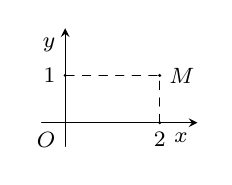
\begin{tikzpicture}[>=stealth,line join=round,line cap=round,font=\footnotesize,scale=0.6]
	\draw[->] (-0.5,0)--(2.8,0) node[below left] {$x$};
	\draw[->] (0,-0.5)--(0,2.0) node[below left] {$y$};
	\draw (0,0) node [below left] {$O$};
	\draw[dashed](2,0)--(2,1)--(0,1);
	\fill 
	(0,1) circle(1pt) node[left]{$1$}
	(2,0) circle(1pt) node[below]{$2$}
	(2,1) circle(1pt) node[right]{$M$};

\end{tikzpicture}}
\loigiai{Từ hình vẽ ta thấy, điểm $M$ biểu diễn cho số phức $z=2+i$.\\
Vậy $\overline{z}=2-i$.}
\end{ex}

\begin{ex}%[Lương Như Quỳnh]%[12-EX-6-2023]%[2D4B2-1]
Cho số phức $z=2+9i$, phần ảo của số phức $z^2$ bằng
\choice
{\True $36$}
{$36i$}
{$18$}
{$9$}
\loigiai{Ta có $z^2=(2+9i)^2=4+36i-81=-77+36i$.\\
Vậy phần ảo của số phức $z^2$ bằng $36$.}
\end{ex}
\begin{ex}%[Lương Như Quỳnh]%[12-EX-6-2023]%[1H3B3-3]
	\immini
	{
		Cho hình chóp $S.ABC$ có $SA \perp (ABC)$, tam giác $ABC$ đều cạnh $a$ và $SA=a$. Tìm góc giữa $SC$ và mặt phẳng $(ABC)$.
		\choice
		{$60^\circ$}
		{\True $45^\circ$}
		{$90^\circ$}
		{$30^\circ$}
	}
	{
\begin{tikzpicture}[>=stealth,line join=round,line cap=round,font=\footnotesize,scale=.6]
\path 
(0,0) coordinate (A)
(1.5,-1.5) coordinate (B)
(5,0) coordinate (C)
($(A)+(90:4)$) coordinate (S)
;
\draw (S)--(A)--(B)--(C)--(S)--(B);
\draw[dashed] (A)--(C) ;
\foreach\p/\g in {S/90, A/180, B/-70, C/0}
\draw[fill=black] (\p) circle (1pt) node[shift=(\g:3mm)] {$\p$};
\end{tikzpicture}
	}
	\loigiai
	{
		\immini
		{
			Vì $SA \perp (ABC)$ nên hình chiếu của $SC$ lên mặt phẳng $(ABC)$ là $AC$.\\
			Do đó góc giữa $SC$ và mặt phẳng $(ABC)$ là góc $\widehat{SCA}$.\\
			Xét $\triangle SAC$ vuông tại $A$, $SA=AC=a$ nên $\triangle SAC$ là tam giác vuông cân tại $A$. Suy ra $\widehat{SCA}= 45^\circ$.\\
			Vậy góc giữa $SC$ và mặt phẳng $(ABC)$ bằng $45^\circ$.
		}
		{
			\begin{tikzpicture}[>=stealth,line join=round,line cap=round,font=\footnotesize,scale=.71]
		\path 
		(0,0) coordinate (A)
		(1.5,-1.5) coordinate (B)
		(5,0) coordinate (C)
		($(A)+(90:4)$) coordinate (S)
		;
		\draw (S)--(A)--(B)--(C)--(S)--(B);
		\draw[dashed] (A)--(C) ;
		\foreach\p/\g in {S/90, A/180, B/-70, C/0}
		\draw[fill=black] (\p) circle (1pt) node[shift=(\g:3mm)] {$\p$};
	\end{tikzpicture}
		}
	}
\end{ex}

\begin{ex}%[Lương Như Quỳnh]%[12-EX-6-2023]%[1D2K5-2]
	Giải bóng đá mini cấp trường của một trường THPT có 16 đội đăng kí tham dự, trong đó có 3 đội 12A{\small 1}, 12A{\small 2} và 12A{\small 3}. Ban tổ chức cho bốc thăm ngẫu nhiên để chia đều 16 đội vào 4 bảng (mỗi bảng 4 đội) để đá vòng loại. Tính xác suất để 3 đội của 3 lớp 12A{\small 1}, 12A{\small 2} và 12A{\small 3} nằm ở 3 bảng khác nhau.
	\choice
	{$\dfrac{3}{56}$}
	{$\dfrac{19}{28}$}
	{$\dfrac{53}{56}$}
	{\True $\dfrac{16}{35}$}
	\loigiai
	{
		Giả sử ta có bốn bảng đấu là $A$, $B$, $C$, $D$.\\
		Mỗi cách chọn 4 đội trong số 16 đội để xếp vào bảng $A$ là một tổ hợp chập 4 của 16 phần tử.\\
		Mỗi cách chọn 4 đội tiếp theo trong số 12 đội còn lại để xếp vào bảng $B$ là một tổ hợp chập 4 của 12 phần tử.\\
		Mỗi cách chọn 4 đội tiếp theo trong số 8 đội còn lại để xếp vào bảng $C$ là một tổ hợp chập 4 của 8 phần tử.\\
		Lúc này, 4 đội cuối cùng sẽ được xếp vào bảng $D$.\\
		Do đó số phần tử của không gian mẫu là $n(\Omega)= \mathrm{C}_{16}^4 \cdot \mathrm{C}_{12}^4 \cdot \mathrm{C}_{8}^4 \cdot \mathrm{C}_{4}^4  = 63063000$.\\
		Gọi $E$ là biến cố \lq\lq 3 đội của 3 lớp 12A{\small 1}, 12A{\small 2} và 12A{\small 3} nằm ở 3 bảng khác nhau\rq\rq.\\
		Số cách xếp 12A{\small 1}, 12A{\small 2} và 12A{\small 3} vào 3 bảng đấu khác nhau là $\mathrm{A}_4^3$.\\		
		Mỗi cách chọn 3 đội trong 13 đội còn lại  để xếp vào bảng có lớp 12A{\small 1} là một tổ hợp chập 3 của 13 phần tử.\\		
		Mỗi cách chọn 3 đội tiếp theo trong 10 đội còn lại  để xếp vào bảng có lớp 12A{\small 2} là một tổ hợp chập 3 của 10 phần tử.\\		
		Mỗi cách chọn 3 đội tiếp theo trong 7 đội còn lại để xếp vào bảng có lớp 12A{\small 3} là một tổ hợp chập 3 của 7 phần tử.\\		
		Lúc này, 4 đội cuối cùng sẽ được xếp vào bảng còn lại.\\
		Suy ra số phần tử của biến cố $E$ là $n(E)= \mathrm{A}_4^3 \cdot \mathrm{C}_{13}^3 \cdot \mathrm{C}_{10}^3 \cdot \mathrm{C}_{7}^4 \cdot \mathrm{C}_{4}^4 = 28828800$.\\
		Vậy xác suất cần tìm là $\mathrm{P}(E)= \dfrac{n(E)}{n(\Omega)}= \dfrac{28828800}{63063000}= \dfrac{16}{35}$.
	}
\end{ex}

\begin{ex}%[Lương Như Quỳnh]%[12-EX-6-2023]%[1H3K5-3]
	\immini
	{
		Cho hình chóp $S.ABCD$ có đáy $ABCD$ là hình vuông cạnh $a$, $SA \perp (ABCD)$ và $SA=\dfrac{a\sqrt{3}}{3}$ (tham khảo hình vẽ bên). Khoảng cách từ $A$ đến mặt phẳng $(SCD)$ là 
		\choice
		{$a$}
		{\True $\dfrac{a}{2}$}
		{$\dfrac{a\sqrt{2}}{2}$}
		{$\dfrac{a\sqrt{3}}{2}$}
	}
	{
		\begin{tikzpicture}[>=stealth,line join=round,line cap=round,font=\footnotesize,scale=.71]
			\path 
			(0,0) coordinate (A)
			(-1.5,-1.5) coordinate (B)
			(4,0) coordinate (D)
			($(B)+(D)-(A)$) coordinate (C)
			($(A)+(90:3)$) coordinate (S)
			;
			\draw (S)--(B)--(C)--(D)--(S)--(C);
			\draw[dashed] (S)--(A)--(D) (A)--(B);
			\foreach\p/\g in {S/90, A/160, B/-90, C/-90, D/0}
			\draw[fill=black] (\p) circle (1pt) node[shift=(\g:3mm)] {$\p$};
		\end{tikzpicture}		
	}
	\loigiai
	{
		\immini
		{
			Gọi $H$ là hình chiếu vuông góc của $A$ lên $SD$ $\Rightarrow AH \perp SD$.\\
			Vì $\heva{&CD \perp AD\\ &CD \perp SA} \Rightarrow CD \perp (SAD) \Rightarrow CD \perp AH$.\\
			Do đó $AH \perp (SCD)$ $\Rightarrow H$ là hình chiếu vuông góc của $A$ lên mặt phẳng $(SCD)$. Suy ra $\mathrm{d} \big( A, (SCD)\big) = AH$.\\
			Xét $\triangle SAC$ vuông tại $A$, đường cao $AH$, ta có
			\begin{eqnarray*}
				\dfrac{1}{AH^2}&=& \dfrac{1}{SA^2}+ \dfrac{1}{AD^2}\\
				&=& \dfrac{9}{3a^2}+ \dfrac{1}{a^2} = \dfrac{4}{a^2}.
			\end{eqnarray*}
			Suy ra $AH=\dfrac{a}{2}$. \\
			Vậy khoảng cách từ $A$ đến mặt phẳng $(SCD)$ bằng $\dfrac{a}{2}$.
		}
		{
			\begin{tikzpicture}[>=stealth,line join=round,line cap=round,font=\footnotesize,scale=.71]
				\path 
				(0,0) coordinate (A)
				(-1.5,-1.5) coordinate (B)
				(4,0) coordinate (D)
				($(B)+(D)-(A)$) coordinate (C)
				($(A)+(90:3)$) coordinate (S)
				($(S)!.3!(D)$) coordinate (H)
				;
				\draw (S)--(B)--(C)--(D)--(S)--(C);
				\draw[dashed] (S)--(A)--(D) (A)--(B) (A)--(H);
				\foreach\p/\g in {S/90, A/160, B/-90, C/-90, D/0, H/45}
				\draw[fill=black] (\p) circle (1pt) node[shift=(\g:3mm)] {$\p$};
				\tkzMarkRightAngle (A,H,D)
			\end{tikzpicture}	
		}
	}
\end{ex}

\begin{ex}%[2D2K6-2]
	Số giá trị nguyên của $x$ thoả $\left( 2^{x^2}-16\right) \left( \log_3 x-4\right) \le 0$ là
	\choice
	{vô số}
	{\True $80$}
	{$17$}
	{$78$}
	\loigiai
	{
		Ta có 
		\[
		\left( 2^{x^2}-16\right) \left( \log_3 x-4\right) \le 0 \Leftrightarrow \heva{&2^{x^2}-16\le 0 \\ & \log_3 x - 4\ge 0} \quad \text{hoặc} \quad \heva{&2^{x^2}-16\ge 0 \\ & \log_3 x - 4\le 0.}
		\]
		Xét hai trường hợp\\
		\textbf{Trường hợp 1.}
		\begin{eqnarray*}
			\heva{&2^{x^2}-16\le 0 \\ & \log_3 x - 4\ge 0} &\Leftrightarrow& \heva{&x^2\le 4\\ & \log_3 x \ge 4}\\
			&\Leftrightarrow& \heva{&-2\le x \le 2\\ &x\ge 81} \quad (\text{không tồn tại}).
		\end{eqnarray*}
		\textbf{Trường hợp 2.}
		\begin{eqnarray*}
			\heva{&2^{x^2}-16\ge 0 \\ & \log_3 x - 4\le 0} &\Leftrightarrow& \heva{&x^2\ge 4\\ & \log_3 x \le 4}\\
			&\Leftrightarrow& \heva{&x\le -2 \text{ hoặc } x\ge 2\\ &0<x\le 81} \Leftrightarrow 2\le x \le 81.
		\end{eqnarray*}
		Vì $x \in \mathbb{Z}$ nên $x\in \{2; 3; 4; \ldots; 81\}$.\\
		Vậy có $80$ giá trị nguyên của $x$ thỏa mãn bài toán.
	}
\end{ex}

\begin{ex}%[Lương Như Quỳnh]%[12-EX-6-2023]%[2D4B4-1]
	Gọi $z_1$, $z_2$ là hai nghiệm của phương trình $z^2-4z+13=0$ và $A$, $B$ lần lượt là hai điểm biểu diễn hai số phức $z_1$, $z_2$ trong mặt phẳng $Oxy$. Diện tích của tam giác $OAB$ bằng
	\choice
	{\True $6$}
	{$12$}
	{$13$}
	{$\dfrac{13}{2}$}
	\loigiai
	{
		\immini
		{
			Ta có
			\[
			z^2-4z+13=0 \Leftrightarrow \hoac{&z_1=2+3i\\ &z_2=2-3i}
			\Rightarrow A(2;3) \text{ và } B(2;-3).
			\]
			Ta thấy hai điểm $A(2;3)$, $B(2;-3)$ đối xứng với nhau qua trục $Ox$.\\
			Gọi $H$ là trung điểm của $AB$. Suy ra $H(2;0)$ và $OH \perp AB$.\\
			Khi đó
			\[
			S_{\triangle OAB}= \dfrac{1}{2} \cdot OH \cdot AB = \dfrac{1}{2} \cdot 2 \cdot 6= 6.
			\]
		}
		{
			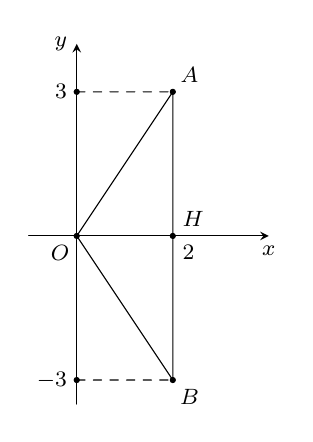
\begin{tikzpicture}[>=stealth,line join=round,line cap=round,font=\footnotesize,scale=.61]
\path 
(2,3) coordinate (A)
(2,-3) coordinate (B)
(0,0) coordinate (O)
;
\draw[->] (-1,0)--(4,0) node[below] {$x$};
\draw[->] (0,-3.5)--(0,4) node[left] {$y$};
\draw (O)--(A)--(B)--(O);
\foreach\p/\g in {O/225, A/45, B/-45}
\draw[fill=black] (\p) circle (1.5pt) node[shift=(\g:3mm)] {$\p$};
\draw[dashed] (0,3)--(A) (0,-3)--(B);
\draw[fill=black] 
(2,0) circle (1.5pt) node[below right] {$2$} node[above right] {$H$}
(0,-3) circle (1.5pt) node[left] {$-3$}
(0,3) circle (1.5pt) node[left] {$3$}
;
\end{tikzpicture}
		}
		
	}
\end{ex}

\begin{ex}%[Lương Như Quỳnh]%[12-EX-6-2023]%[2D3K3-1]
	Cho hàm số $y=f(x)$ có đạo hàm liên tục trên $\mathbb{R}$ và thoả mãn $\left( x^3+4x\right) f'(x)= -\left( 3x^2+4\right) f(x) +4$, $\forall\, x\in \mathbb{R}$. Diện tích hình phẳng giới hạn bởi các đường $y=f(x)$, hai trục toạ độ và $x=2$ là
	\choice
	{$\dfrac{2\pi}{3}$}
	{\True $\dfrac{\pi}{2}$}
	{$\dfrac{4\pi}{3}$}
	{$2\pi$}
	\loigiai
	{
		$\forall\, x\in \mathbb{R}$, ta có
		\begin{eqnarray*}
			\left( x^3+4x\right) f'(x)= -\left( 3x^2+4\right) f(x) +4 &\Rightarrow& \left( x^3+4x\right) f'(x)+ \left( 3x^2+4\right) f(x)= 4\\
			&\Rightarrow& \left[ \left( x^3+4x\right) f(x)\right]' = 4\\
			&\Rightarrow& \left( x^3+4x\right) f(x) = 4x+C.
		\end{eqnarray*}
		Mặt khác, với $x=0$ suy ra $C=0$ và do hàm $f(x)$ liên tục nên $f(x)= \dfrac{4}{x^2+4}$.\\
		Diện tích hình phẳng cần tìm là 
		\[
		S= \displaystyle\int\limits_0^2 \left| \dfrac{4}{x^2+4}\right| \mathrm{\, d}x =  \displaystyle\int\limits_0^2 \dfrac{4}{x^2+4} \mathrm{\, d}x.
		\]
		Đặt $x=2\tan t$, ta có $\mathrm{d}x= \dfrac{2}{\cos^2 t} \mathrm{\, d} t$.\\
		Đổi cận: với $x=0$ thì $t=0$, với $x=2$ thì $t=\dfrac{\pi}{4}$. Do đó
		\begin{eqnarray*}
			S=\displaystyle\int\limits_0^2 \dfrac{4}{x^2+4} \mathrm{\, d}x&=& \displaystyle\int\limits_0^{\tfrac{\pi}{4}} \dfrac{4}{4\tan^2 t+4} \cdot \dfrac{2}{\cos^2 t} \mathrm{\, d}t\ = \displaystyle\int\limits_0^{\tfrac{\pi}{4}} \cos^2 t \cdot \dfrac{2}{\cos^2 t} \mathrm{\, d}t\\
			&=& \displaystyle\int\limits_0^{\tfrac{\pi}{4}} 2 \mathrm{\, d} t = 2t\Big|_0^{\tfrac{\pi}{4}}= \dfrac{\pi}{2}.
		\end{eqnarray*}
	}
\end{ex}

\begin{ex}%[Lương Như Quỳnh]%[12-EX-6-2023]%[2D3K3-3]
	\immini
	{
		Một cái ly làm bằng thủy tinh, có hình dạng là khối nón cụt và các kích thước như hình vẽ bên. Phần rỗng bên trong có thiết diện qua trục là parabol. Thể tích khối thủy tinh bằng bao nhiêu?
		\choice
		{$\dfrac{43}{4} \pi$}
		{$\dfrac{55}{4} \pi$}
		{\True $\dfrac{33}{4} \pi$}
		{$\dfrac{65}{4} \pi$}
	}
	{
		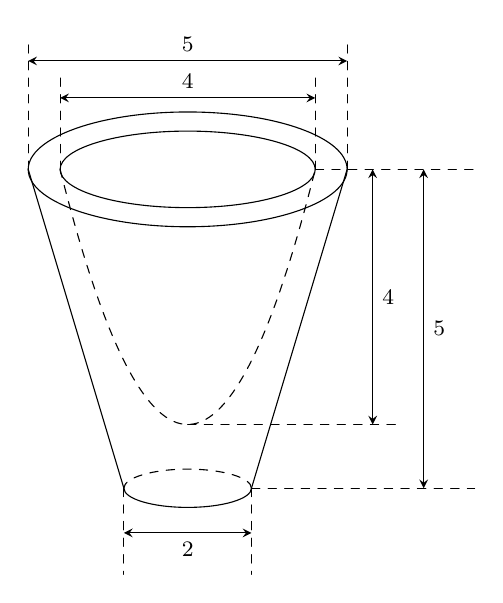
\begin{tikzpicture}[>=stealth,line join=round,line cap=round,font=\footnotesize,scale=.81]
	\draw (2.5,4) arc (0:360: 2.5 and .9);
	\draw (2,4) arc (0:360: 2 and .6);
	\draw[dashed] (1,-1) arc (0:180:1 and .3);
	\draw (1,-1) arc (0:-180:1 and .3);
	\draw (2.5,4)--(1,-1) (-1,-1)--(-2.5,4);
	\draw[smooth, samples=100, domain=-2:2, dashed] plot (\x, {(\x)^2});
	\draw[dashed]
	(2.5,4)--(2.5,6) (-2.5,4)--(-2.5,6)
	(2,4)--(2,5.5) (-2,4)--(-2,5.5)
	(0,0)--(3.3,0) (2,4)--(4.5,4) (1,-1)--(4.5,-1)
	(1,-1)--(1,-2.35) (-1,-1)--(-1,-2.35)
	 ;
	 \draw[<->] (-2.5,5.7)--(2.5,5.7) node[above, midway] {$5$};
	 \draw[<->] (-2,5.12)--(2,5.12) node[above, midway] {$4$};
	 \draw[<->] (-1,-1.7)--(1,-1.7) node[below, midway] {$2$};
	 \draw[<->] (2.9,0)--(2.9,4) node[right, midway] {$4$};
	 \draw[<->] (3.7,-1)--(3.7,4) node[right, midway] {$5$};
\end{tikzpicture}
	}
	\loigiai
	{
		\immini
		{
			Chọn hệ trục toạ độ như hình vẽ bên.\\
			Gọi $V_1$, $V_2$, $V$ lần lượt là thể tích của khối nón cụt, thể tích phần rỗng bên trong ly và thể tích khối thủy tinh.\\
			Ta có toạ độ các điểm $A\left( \dfrac{5}{2}; 4\right)$, $B(1;-1)$, nên đường thẳng $AB$ cắt trục $Oy$ tại điểm $I\left( 0; -\dfrac{13}{3}\right)$.\\
			Thể tích khối nón đỉnh $I$, đường sinh $IA$ là
			\[
			V_a= \dfrac{1}{3} \pi \cdot \left( \dfrac{5}{2}\right)^2 \cdot \dfrac{25}{3}= \dfrac{625}{36} \pi.
			\]
			Thể tích khối nón đỉnh $I$, đường sinh $IB$ là
			\[
			V_b= \dfrac{1}{3} \pi \cdot 1^2 \cdot \dfrac{10}{3}= \dfrac{10}{9} \pi.
			\]
			Suy ra $V_1= V_a-V_b= \dfrac{625}{36}\pi - \dfrac{10}{9}\pi= \dfrac{65}{4}\pi$.\\
			}
		{
				\begin{tikzpicture}[>=stealth,line join=round,line cap=round,font=\footnotesize,scale=.81]
				\draw (2.5,4) arc (0:360: 2.5 and .9);
				\draw (2,4) arc (0:360: 2 and .6);
				\draw[dashed] (1,-1) arc (0:180:1 and .3);
				\draw (1,-1) arc (0:-180:1 and .3);
				\draw (2.5,4)--(1,-1)--(0,-4.33)--(-1,-1)--(-2.5,4);
				\draw[smooth, samples=100, domain=-2:2, dashed] plot (\x, {(\x)^2});
%				\draw[dashed]
%				(2.5,4)--(2.5,6) (-2.5,4)--(-2.5,6)
%				(2,4)--(2,5.5) (-2,4)--(-2,5.5)
%				(0,0)--(3.3,0) (2,4)--(4.5,4) (1,-1)--(4.5,-1)
%				(1,-1)--(1,-2.35) (-1,-1)--(-1,-2.35)
%				;
%				\draw[<->] (-2.5,5.7)--(2.5,5.7) node[above, midway] {$5$};
%				\draw[<->] (-2,5.12)--(2,5.12) node[above, midway] {$4$};
%				\draw[<->] (-1,-1.7)--(1,-1.7) node[below, midway] {$2$};
%				\draw[<->] (2.9,0)--(2.9,4) node[right, midway] {$4$};
%				\draw[<->] (3.7,-1)--(3.7,4) node[right, midway] {$5$};
				\draw[->] (-3.5,0)--(4,0) node[below] {$x$};
				\draw[->] (0,-5)--(0,5.5) node[left] {$y$};
				\draw[dashed] 
				(-1,0)--(-1,-1) (0,-1)--(1,-1)--(1,0)
				(-2.5,0)--(-2.5,4)--(2.5,4)--(2.5,0)
				(2,0)--(2,4) (-2,0)--(-2,4)
				;
				\draw[fill=black]
				(-2.5,0) circle (1pt) node[shift=(-120:4mm)] {$-\tfrac{5}{2}$}
				(2.5,0) circle (1pt) node[below] {$\tfrac{5}{2}$}
				(-1,0) circle (1pt) node[above] {$-1$}
				(1,0) circle (1pt) node[above] {$1$}
				(0,4) circle (1pt) node[above left] {$4$}
				(0,-1) circle (1pt) node[left] {$-1$}
				(0,-4.33) circle (1pt) node[left] {$-\tfrac{13}{3}$} node[right] {$I$}
				(2.5,4) circle (1pt) node[right] {$A$}
				(1,-1) circle (1pt) node[right] {$B$}
				(2,4) circle (1pt)
				(2,0) circle (1pt) node[below] {$2$}
				(-2,0) circle (1pt) node[below] {$-2$}
				(0,0) circle (1pt) node[below left] {$O$}
				 ;
			\end{tikzpicture}
		}
		\noindent Mặt khác, đường parabol có đỉnh là $O(0;0$), đi qua điểm $(2;4)$ nên có phương trình là $y=x^2$.\\
		Do đó thể tích phần rỗng bên trong ly là
		\begin{eqnarray*}
			V_2&=& \pi \displaystyle\int\limits_0^4 y \mathrm{\, d}y =\pi \left. \dfrac{y^2}{2}\right|_0^4 = 8\pi
		\end{eqnarray*}
		Vậy thể tích khối thuỷ tinh cần tìm là
		\[
		V= V_1-V_2= \dfrac{65}{4}\pi- 8\pi = \dfrac{33}{4}\pi.
		\]
	}
\end{ex}

\begin{ex}%[Lương Như Quỳnh]%[12-EX-6-2023]%[2H3K2-6]
Trong KG $Oxyz$, cho điểm $A(0;1;2)$ và đường thẳng $d\colon \dfrac{x-4}{2}=\dfrac{y-2}{-1}=\dfrac{z-1}{-2}$. Gọi $(P)$ là mặt phẳng chứa $d$ và cách $A$ một khoảng lớn nhất. Khoảng cách từ điểm $M(5;-1;3)$ đến $(P)$ bằng
\choice
{\True $ \dfrac{2}{3} $}
{$ \dfrac{7}{3}$}
{$ \dfrac{1}{3}$}
{$ 1$}
\loigiai{
\begin{center}
\begin{tikzpicture}[font=\footnotesize,line cap=round,line join=round, >=stealth,scale=1.8]
	\def \a{-2} \def \b{-1}\def \c{5} \def \h{4} 
	\path (.5,.7)coordinate(M) 	
	+(\a,\b)coordinate(Q)
	+(\c,0)coordinate(N)
	($(N)+(Q)-(M)$)coordinate(P);
	\coordinate (d) at ($(M)+(-15:.5)$);
	\coordinate (D') at ($(M)+(-15:3)$);
	\coordinate (I) at ($(M)+(-15:1.5)$);
	\coordinate (H) at ($(I)+(10:1.2)$);
	\coordinate (A) at ($(H)+(90:.8)$);
	\draw (M)--(Q)--(P) (d)--(D') (A)--(I)--(H)--cycle;	
	\foreach \x/\g in{I/-120,A/0,H/-45}
	\fill[black](\x) circle (1pt)($(\x)+(\g:2.5mm)$) node{\small $\x$};
	\node at (d) [above right]{$d$};
	\draw[-] ($(Q)!6mm!(P)$) to[bend right=45] node[pos=.5,left]{$P$} ($(Q)!6mm!(M)$);	
\end{tikzpicture}
\end{center}
Gọi $H$, $I$ lần lượt là hình chiếu của $A$ lên $(P)$ và đường thẳng $d$.\\
Khi đó $\mathrm{d}(A,(P))=A H \leq A I$.\\
Do đó $\mathrm{d}(A,(P))_{\max }=A I \Leftrightarrow(P)$ chứa đường thẳng $d$ và nhận $\overrightarrow{A I}$ là véc-tơ pháp tuyến.\\
%Tìm $I$: 
Do $I \in d \Rightarrow I(4+2 t ; 2-t ; 1-2 t) \Rightarrow \overrightarrow{A I}=(2 t+4 ; 1-t ;-1-2 t)$. \\
Vì $A I \perp d \Leftrightarrow \overrightarrow{A I} \perp \overrightarrow{u_{d}} \Leftrightarrow \overrightarrow{A I} \cdot \overrightarrow{u_{d}}=0 \Leftrightarrow 2(2 t+4)-1(1-t)-2(-2 t-1)=0 \Leftrightarrow t=-1$.\\
Suy ra $I(2 ; 3 ; 3)$ và $\overrightarrow{A I}=(2 ; 2 ; 1)$. Khi đó phương trình $(P)\colon 2 x+2 y+z-13=0$.\\
Khoảng cách từ điểm $M(5;-1;3)$ đến $(P)$ bằng $\mathrm{d}(M,(P))=\dfrac{|2\cdot 5+2(-1)+3-13|}{\sqrt{2^{2}+2^{2}+1^{2}}}=\dfrac{2}{3}$.
}
\end{ex}
\begin{ex}%[Lương Như Quỳnh]%[12-EX-6-2023]%[2D1K1-3]
Có bao nhiêu giá trị nguyên của tham số $m \in[-2023 ; 2023]$ để hàm số $y=\left|\dfrac{x-10}{x-m}\right|$ đồng biến trên $(-5 ; 5]$?
\choice
{$ 2017$}
{$ 2019$}
{$ 2018$}
{\True $ 4$}
\loigiai{
Xét hàm số $h(x)=\dfrac{x-10}{x-m}$ với tập xác định $\mathscr{D}=(-\infty ; m) \cup(m ;+\infty)$. Khi đó $y=|h(x)|$.\\
Ta có $h'(x)=\dfrac{10-m}{(x-m)^{2}}$.\\
Nếu $10-m>0 \Leftrightarrow m<10$, khi đó hàm số $h(x)$ đồng biến trên $(-\infty ; m) ;(m ;+\infty)$.\\
Để hàm số $y=|h(x)|$ đồng biến trên $(-5 ; 5]$ thì điều kiện là
\[\hoac{
&\heva{&m \leq-5 \\&h(-5)>0}\Leftrightarrow \heva{&m \leq-5 \\&\dfrac{15}{m+5}>0} \Leftrightarrow \heva{&m \leq-5 \\ &m>-5} \Rightarrow m \in \varnothing \\ 
& \heva{&m>5\\&h(-5)>0} \Leftrightarrow \heva{&m>5 \\ &\dfrac{15}{m+5}>0} \Leftrightarrow \heva{&m>5 \\ &m>-5} \Rightarrow m>5.}\]
Kết hợp điều kiện ta có $5<m<10 \Rightarrow m \in\{6,7,8,9\}$.\\
Nếu $10-m<0 \Leftrightarrow m>10$, khi đó hàm số $h(x)$ nghịch biến trên $(-\infty ; m) $, $(m ;+\infty)$.\\
Để hàm số $y=|h(x)|$ đồng biến trên $(-5 ; 5]$ thì điều kiện là
\[\hoac{&\heva{&m \leq - 5\\& h(- 5)<0}
\Leftrightarrow \heva{& m\leq - 5\\&\dfrac{15}{m+5} < 0}
\Leftrightarrow \heva{&m \leq-5 \\&m<-5} \Rightarrow m<-5\text{ (loại)} \\
&\heva{&m>5\\&h(-5)<0}\Leftrightarrow \heva{&m > 5\\&\dfrac{15}{m+5}<0}\Leftrightarrow \heva{&m>5\\&m<-5} \Rightarrow m \in \varnothing.}\]
Vậy có $4$ giá trị $m$ thỏa mãn yêu cầu bài toán.
}
\end{ex}
\begin{ex}%[Lương Như Quỳnh]%[12-EX-6-2023]%[2H2K1-4]
\immini{Cho một cổ vật hình trụ có chiều cao đo được là $81$ cm, do bị hư hại nên khi tiến hành đo đạc lại thu được $A B=50$ cm, $B C=70$ cm, $C A=80$ cm, với $A$, $B$, $C$ thuộc đường tròn nắp trên như hình vẽ. Thể tích khối cổ vật ban đầu gần nhất với số nào sau đây?
\choice
{$6{,}56$ m$^3$}
{\True $0{,}42$ m$^3$}
{$1{,}03$ m$^3$}
{$0{,}43$ m$^3$}}
{
\definecolor{ecru}{rgb}{0.76, 0.7, 0.5}
\begin{tikzpicture}[line join=round, line cap=round,scale=1,transform shape]
%\clip (-3,-3) rectangle (3,4);
\tikzset{co_vat/.pic={
\def\N{ 
($(0,1.75) + (50:1.55 and .6)$)  arc (50:-230:1.55 cm and .6cm)
..controls +(-10:.1) and +(-170:.1) ..(-.4,2.2)
..controls +(-50:.2) and +(150:.2) ..(0,2.05)
..controls +(10:.2) and +(-150:.3) ..(.8,2.25) --cycle
;
}
\draw[ecru!70!black]\N;
\fill[ecru!80] \N;

\path ($(0,-.4)+(0,1.75) + (180:1.55 and .6)$) coordinate (C')
($(0,-3.5)+(0,1.75) + (0:1.55 and .6)$) coordinate (M)
;

\def\T{ 
(1.55,1.75) arc (0:-180:1.55 cm and .6cm)--(C')..controls +(-30:1) and +(110:1) ..(0,0)
..controls +(-70:1.3) and +(-65:1.1) ..(-1.5,-1)--(-1.5,-1.8)--(-1.5,-1.8) arc (-180:-68:1.55 cm and .6cm)..controls +(75:.2) and +(-145:.1) ..(.8,-2.1)
..controls +(115:.2) and +(-145:.1) ..(.77,-1.7)--(.8,-1.73)
..controls +(35:.2) and +(175:.2) ..(1.3,-1.4)
..controls +(35:.1) and +(175:.1) ..(1.5,-1.2)--cycle
;
}
\draw[ecru!70!black]\T;
\fill[ecru] \T;

\def\B{ 
(C')..controls +(-30:1) and +(110:1) ..(0,0)
..controls +(-70:1.3) and +(-65:1.1) ..(-1.5,-1)
..controls +(80:.9) and +(-45:.9)..cycle
;
}
\draw[ecru!70!black]\B;
\fill[ecru!80] \B;

\draw ($(0,1.75) + (-64:1.55 and .6)$) node[below]{\footnotesize $B$}--($(0,1.75) + (40:1.55 and .6)$) node[above]{\footnotesize $A$}--($(0,1.75) + (180:1.55 and .6)$) node[left]{\footnotesize $C$}--cycle;
}}

\path
(0,0)pic[scale=1]{co_vat};
\end{tikzpicture}
}
\loigiai{
Xét tam giác $A B C$ ta có
\begin{itemize}
\item Nửa chu vi $P=\dfrac{50+70+80}{2}=100$ cm.
\item $S_{ABC}=\sqrt{P(P-AB)(P-AC)(P-BC)} \approx 1732{,}05$ cm$ ^2 $.
\item Bán kính đường tròn ngoại tiếp $R=\dfrac{abc}{4S}=\dfrac{50\cdot 70\cdot 80}{4S} \approx 40{,}41454$ cm.
\end{itemize}
Thể tích của khối cổ vật là $V=S \cdot h=\pi R^{2} \cdot h \approx 415633{,}1$ cm$^3\approx 0{,}4156331$ m$^3$.
}
\end{ex}
\begin{ex}%[Lương Như Quỳnh]%[12-EX-6-2023]%[2H1G3-2]
Cho tứ diện $ABCD$ có $AB=a$, $AC=a \sqrt{5}$, $\widehat{DAB}=\widehat{CBD}=90^{\circ}$, $\widehat{A B C}=135^{\circ}$. Biết góc giữa hai mặt phẳng $(ABD)$ và $(BCD)$ bằng $30^{\circ}$. Thể tích khối tứ diện $ABCD$ bằng
\choice
{$\dfrac{a^{3}}{\sqrt{2}}$}
{$\dfrac{a^{3}}{3 \sqrt{2}}$}
{$\dfrac{a^{3}}{2 \sqrt{3}}$}
{\True $\dfrac{a^{3}}{6}$}
\loigiai{
\begin{center}
\begin{tikzpicture}[font=\footnotesize,line cap=round,line join=round, >=stealth,scale=1]
	\def \a{2} \def \b{-1}\def \c{5} \def \h{5} 
	\path (0,0)coordinate(H) 	
	+(\a,\b)coordinate(E)
	+(\c,0)coordinate(B)
	($(H)+(B)-(E)$)coordinate(F)
	($(E)!2.2!(B)$)coordinate(C)
	($(B)!1.3!(F)$)coordinate(D)
	;
	\coordinate (A) at ($(H)+(90:\h)$);
	\draw (A)--(H)--(E)--(B)--cycle (B)--(C)--(A)--(E);	
	\draw[dashed] (D)--(C) (A)--(D)--(B) (H)--(F)--(A);
	\foreach \x/\g in{A/180,E/-90,D/180,H/180,F/45,C/0,B/-90}
	\fill[black](\x) circle (1pt)($(\x)+(\g:2.5mm)$) node{\small $\x$};
	\node at (3,2) [above right]{$a$};
	\node at (5,2.7) [above right]{$a\sqrt{5}$};
	\node at (6,0) [above right]{$a\sqrt{2}$};
	\draw[-] ($(B)!5mm!(C)$) to[bend right=45]($(B)!5mm!(A)$);	
	\draw pic[draw=black, angle eccentricity=2, angle radius=0.25cm]
	{right angle=D--B--C};
\end{tikzpicture}
\end{center}
Gọi $BC=x$ $(x>0)$.\\
Áp dụng định lý hàm số cô-sin trong tam giác $ABC$ ta có
\[5 a^{2}=a^2+x^2-2 a x \cdot \cos 135^{\circ}\Leftrightarrow x^2+\sqrt{2} a x-4 a^2=0 \Leftrightarrow \hoac{&x=a \sqrt{2} \\ &x=-2 \sqrt{2} a.}\]
Từ $A$ kẻ $AF \perp BD$ tại $F$, kẻ $AE \perp BC$ tại $E$, từ $F$ kẻ song song với $B C$ và $E$ kẻ song song với $B D$ cắt nhau tại $H$ nên $((ABD),(BCD))=(AF,HF)=\widehat{AFH}=30^{\circ}$.\\
Ta có $BD \perp AF$, $BD \perp HF$ nên $BD \perp(AHF)$ suy ra $AH \perp BD$.\\
Ta có $BC \perp A E$, $BD \perp E H$ nên $BC \perp(AHE)$ suy ra $BC \perp AH$.\\
Nên $AH \perp(BCD)$.\\
Ta có $\widehat{ABC}=135^{\circ} \Rightarrow \widehat{ABE}=45^{\circ}$.\\
Suy ra tam giác $AEB$ vuông tại $E$ nên $EB=EA=\dfrac{a}{\sqrt{2}}$.\\
Do $BEHF$ là hình chữ nhật nên $EB=HF=\dfrac{a}{\sqrt{2}}$.\\
Xét tam giác $AHF$ vuông tại $H$ nên $AH=HF \cdot \tan \widehat{AFH} =\dfrac{a}{\sqrt{2}} \cdot \tan 30^{\circ}=\dfrac{a}{\sqrt{2}} \cdot \dfrac{\sqrt{3}}{3}=\dfrac{a \sqrt{6}}{6}$.\\
Xét tam giác $AHE$ vuông tại $E$ nên $HE=BF=\sqrt{AE^{2}-AH^{2}}=\sqrt{\dfrac{a^{2}}{2}-\dfrac{a^{2}}{6}}=\dfrac{a}{\sqrt{3}}$.\\
Xét tam giác $ABD$ vuông tại $A$ nên $AB^{2}=BF \cdot BD \Rightarrow BD=\dfrac{A B^{2}}{B F}=\dfrac{a^{2}}{\dfrac{a}{\sqrt{3}}}=a^{2} \cdot \dfrac{\sqrt{3}}{a}=a \sqrt{3}$.\\
Thể tích của khối chóp $ABCD$ là $V=\dfrac{1}{6} \cdot AH \cdot BD \cdot BC=\dfrac{1}{6} \cdot \dfrac{a\sqrt{6}}{6} \cdot a \sqrt{2} \cdot a \sqrt{3}=\dfrac{a^{3}}{6}$.
}
\end{ex}
\begin{ex}%[Lương Như Quỳnh]%[12-EX-6-2023]%[2H3G1-4]
Trong KG $Oxyz$, cho hai điểm $A(0;0;10)$ và $B\left(3;4;\dfrac{19}{2}\right)$. Xét các điểm $M$ thay đổi sao cho tam giác $OAM$ không phải là tam giác nhọn và có diện tích bằng $20$. Giá trị nhỏ nhất của độ dài đoạn thẳng $MB$ thuộc khoảng nào dưới đây?
\choice
{$(5;10)$}
{$(3;5)$}
{$\left(\dfrac{3}{2};3\right)$}
{\True $\left(0;\dfrac{3}{2}\right) $}
\loigiai{
\begin{center}
\begin{tikzpicture}[scale=.5, font=\footnotesize, line join=round, line cap=round,>=stealth] 
	\def\xmin{-8} \def\xmax{8}
	\def\ymin{-4} \def\ymax{13} 
	%\draw[color=gray!50,dashed] (\xmin,\ymin) grid (\xmax,\ymax); 
	\draw[->] (4,0)--(\xmax,0) node [below]{$y$};
	\draw[->] (0,10)--(0,\ymax) node [left]{$z$};
	\draw[dashed] (0,0)--($(0,0)+(-120:1.8)$);
	\draw[->] ($(0,0)+(-120:1.7)$)--($(0,0)+(-120:3.7)$) node [left]{$x$};
	\draw ($(0,0)+(-120:1.7)$) circle (.5pt) node [below right]{$4$};
	\draw[dashed] (0,6.5)--($(0,6.5)+(-20:3.05)$) circle (.5pt) node [above]{$M$}--(0,10);
	\draw[dashed] (0,0)--($(0,0)+(-20:3.05)$) circle (.5pt)
	($(-1.2,0)+(-20:3.7)$)--($(-4.2,0)+(-20:3.7)$)circle (.5pt) node [left]{$3$};
	\draw ($(0,6.5)+(-20:3.05)$)--($(0,6.5)+(-20:3.7)$) circle (.5pt) node [below left]{$B$};
	\draw[dashed] ($(0,0)+(-20:3.05)$)--($(0,0)+(-20:3.7)$) circle (.5pt);%1
	\draw[dashed] ($(0,6.5)+(-20:3.7)$)--($(0,0)+(-20:3.7)$)
	($(0,0)+(-20:3.7)$)--(4,0) ($(0,0)+(-20:3.7)$)--($(-1.2,0)+(-20:3.7)$);%2
	\draw[dashed](0,0)--($(0,6.5)+(-20:3.05)$);
	\node at (0,0) [left]{$O$};
	\draw[dashed](4,0)  circle (.5pt) node [above right]{$4$}--(0,0)--(0,10)node [right]{$A$};
	\draw[dashed,red] (4,0) arc (0:180:4 cm and 1.5cm);
	\draw[red] (4,0) arc (0:-180:4 cm and 1.5cm);
	\draw[dashed,red,shift={(0,6.5)}] (4,0) arc (0:180:4 cm and 1.5cm);
	\draw[red,shift={(0,6.5)}] (4,0) arc (0:-180:4 cm and 1.5cm);
	\draw[red,shift={(0,10)}] (4,0) arc (0:360:4 cm and 1.5cm);
	\draw[fill=black] (0,10) circle (.5pt) node[left]{\footnotesize $10$};
	\draw[fill=black] (-2.5,4) node[right]{\footnotesize $(C)$};
	\draw[fill=black] (0,6.5) circle (.5pt) node[left]{\footnotesize $\frac{19}{2}$};
	\draw[fill=black] (0,6.5) node[above right]{\footnotesize $I$};
	\draw[blue] (-4,0)--(-4,10) (4,0)--(4,10);
\end{tikzpicture}
\end{center}
Có $S_{\triangle OAM}=\dfrac{1}{2} OA \cdot \mathrm{d}(M,Oz)=\dfrac{1}{2} \cdot 10\cdot \mathrm{d}(M,Oz)=20 \Leftrightarrow \mathrm{d}(M,Oz)=4$. \\
Suy ra tập hợp các điểm $M$ là hình trụ có trục là $O z$ và bán kính $r=4$.\\
Xét mặt phẳng $(\alpha)$ đi qua $B$ và vuông góc trục $Oz$, cắt hình trụ theo đường tròn $(C)$ có tâm là điểm $I\left(0;0;\dfrac{19}{2}\right)$.\\
Dễ thấy điểm $B$ nằm ngoài $(C)$ và $BM$ ngắn nhất khi $M\in(C)$ nằm trên mặt phẳng $(\alpha)$.\\
Có $\min BM=BI-r=\sqrt{3^{2}+4^{2}+0^{2}}-4=5-4=1$.
}
\end{ex}
\begin{ex}%[Lương Như Quỳnh]%[12-EX-6-2023]%[2D4G5-1]
Cho các số phức $z$, $w$, $u$ thỏa $|z-4+2 i|=\left|2 z+\overline{z}\right|$, $\dfrac{w-8-10 i}{w-6-10i}$ là số thuần ảo và $|u+1-2i|=|u-2+i|$. Giá trị nhỏ nhất của $T=|u-z|+\left|\overline{u}-\overline{w}\right|$ thuộc khoảng nào sau đây?
\choice
{$(0;5]$}
{\True $(5;8)$}
{$[8;10)$}
{$[10 ;+\infty)$}
\loigiai{
Giả sử các số phức $z$, $w$, $u$ lần lượt có điểm biểu diễn là $M$, $N$, $P$ và $\overline{w}$, $\overline{u}$ lần lượt có điểm biểu diễn là $N'$, $P'$ ($N'$, $P'$ lần lượt đối xứng với $N$, $P$ qua trục $x'Ox$).\\
Dễ thấy $M \in(P)\colon y=2 x^{2}+2 x-5$, $N \in(C)$ có tâm $I(7;10)$ và $R=1$ (bỏ điểm $J(6 ; 10)$).\\
Suy ra $N'\in\left(C'\right)$ có tâm $I'(7 ;-10)$ và $R'=1$.\\
$P \in(d)\colon x-y=0$. Suy ra $P' \in\left(d'\right)\colon x+y=0$.\\
Khi đó $T=|u-z|+\left|\overline{u}-\overline{w}\right|=MP+P'N'=MP+PN$.\\
Dễ thấy để $T$ nhỏ nhất thì $M$ thuộc nhánh phải của $(P)$ và nằm cùng phía với đường tròn $(C)$ so với đường thẳng $d$.\\
Gọi $N''$ là ảnh của $N$ qua phép đối xứng trục $d$ $\left(N'' \in\left(C''\right)\right)$ là ảnh của $(C)$ qua phép đối xứng trục $d $; $\left(C''\right)$ có tâm $I''(10;7)$, bán kính $R''=1$.
\begin{center}
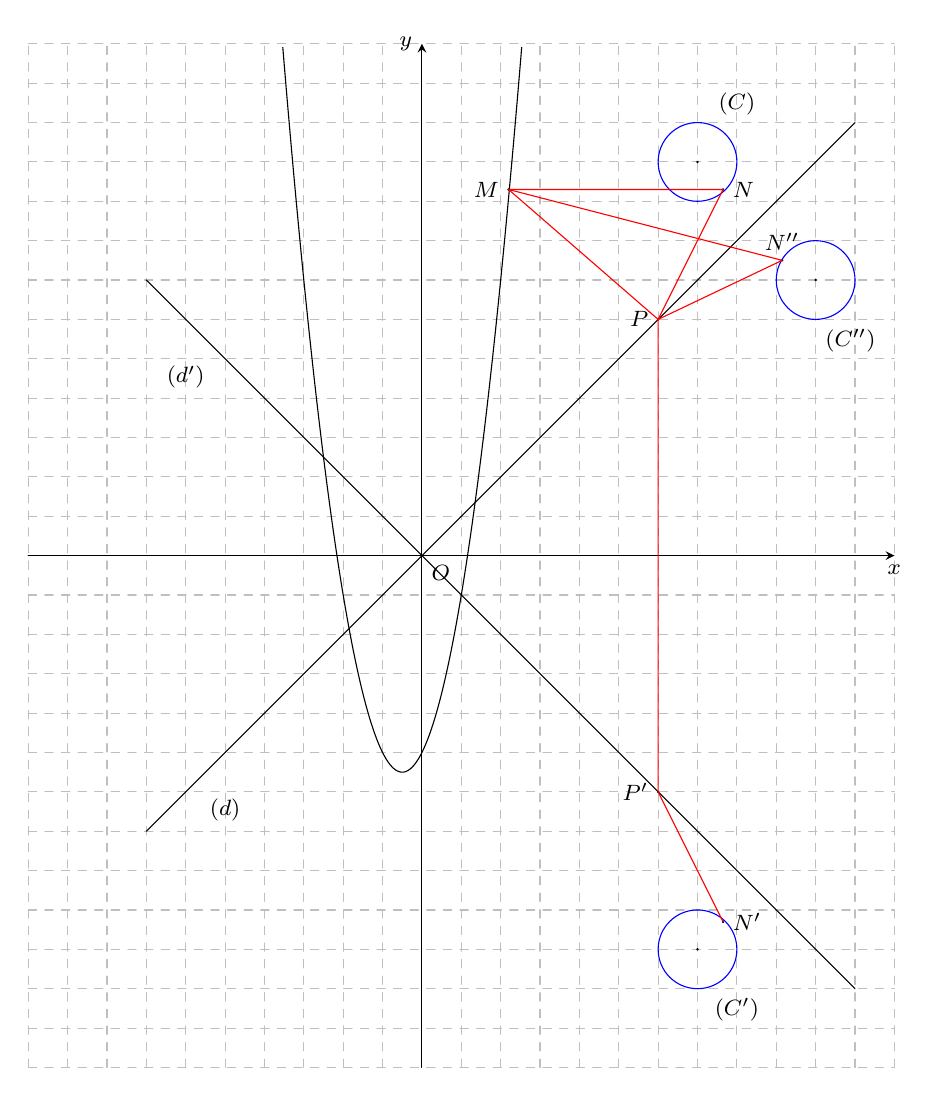
\begin{tikzpicture}[scale=.5, font=\footnotesize, line join=round, line cap=round,>=stealth] 
	\def\xmin{-10} \def\xmax{12}
	\def\ymin{-13} \def\ymax{13} 
	\draw[color=gray!50,dashed] (\xmin,\ymin) grid (\xmax,\ymax); 
	\draw[->] (\xmin,0)--(\xmax,0) node [below]{$x$};
	\draw[->] (0,\ymin)--(0,\ymax) node [left]{$y$};
	\node at (0,0) [below right]{$O$};
	\node at (-6,4) [above]{$(d')$};
	\node at (-5,-7) [above]{$(d)$};
	\node at (8,-11) [below]{$(C')$};
	\node at (8,12) [below]{$(C)$};
	\node at (10,6) [below right]{$(C'')$};
	\draw[fill=black] (7,10) circle (.5pt);
	\draw[fill=black] (7,-10) circle (.5pt);
	\draw[fill=black] (10,7) circle (.5pt);
	\draw[fill=black] (2.2,9.3) circle (.5pt) node[left]{\footnotesize $M$};
	\draw[fill=black] (7.65,9.3) circle (.5pt) node[right]{\footnotesize $N$};
	\draw[fill=black] (6,6) circle (.5pt) node[left]{\footnotesize $P$};
	\draw[fill=black] (6,-6) circle (.5pt) node[left]{\footnotesize $P'$};
	\draw[fill=black] (7.65,-9.3) circle (.5pt) node[right]{\footnotesize $N'$};
	\draw[fill=black] (9.15,7.5) circle (.5pt) node[above]{\footnotesize $N''$};
	\clip (\xmin+0.1,\ymin+0.1) rectangle (\xmax-0.1,\ymax-0.1);
	\draw[smooth,samples=300,domain=-5:5] plot(\x,{2*(\x)^2+2*(\x)-5});
	\draw[smooth,samples=300,domain=-7:11] plot(\x,{(\x)});
	\draw[smooth,samples=300,domain=-7:11] plot(\x,{(-\x)});
	\draw[blue] (7,10) circle (1 cm);
	\draw[blue] (7,-10) circle (1 cm);
	\draw[blue] (10,7) circle (1 cm);
	\draw[red] (2.2,9.3)--(7.65,9.3)--(6,6)--cycle (6,-6)--(7.65,-9.3);
	\draw[red] (6,6)--(6,-6) (2.2,9.3)--(9.15,7.5)--(6,6);
\end{tikzpicture}
\end{center}
Khi đó $T=MP+PN=M P+PN''\geq M N''$. Dấu \lq\lq =\rq\rq\, khi $M$, $P$, $N''$ thẳng hàng $\left(M \in(P),\,N'' \in\left(C''\right)\right)$.\\
Gọi $\left(C_1\right)$ là đường tròn tâm $I''(10 ; 7)$, bán kính $r=m$. (tăng bán kính $r=m$ để $\left(C_1\right)$ tiếp xúc $(P)$, khi đó $r-1=m-1$ là đoạn ngắn nhất từ một điểm $M \in(P)$ và $N'' \in\left(C''\right)$).\\
Có $\left(C_1\right)\colon (x-10)^{2}+(y-7)^2=m^{2}$.\\
Tọa độ giao điểm của $\left(C_1\right)$ và $(P)$ là nghiệm của hệ: {\bf (tìm giao điểm thay cho tiếp xúc)}
\[\heva{&(x - 10)^2+(y-7)^2= m^2 \\&y=2x^2+2x-5}
\Leftrightarrow \heva{
&m=\sqrt{(x-10)^{2}+\left(2 x^2+2 x-12\right)^2}\quad(*) \\
&y=2 x^{2}+2 x-5.}\]
%Sử dụng MODE $7$, (với $x \in[1;10]$), tìm được giá trị nhỏ nhất của $m$ là $8$ đạt khi $x=2$.\\
Xét hàm số $ g(x)=\sqrt{(x-10)^{2}+\left(2 x^2+2 x-12\right)^2} $, $x \in[1;10]$.\\
Ta tìm được $ \min \limits_{[1;10]} g(x)=8$ đạt khi $x=2$.\\
Suy ra $ \min m=8$ đạt khi $x=2$.\\
Vậy $\min MN''=m-R''=8-1=7 \in(5;8)$.
}
\end{ex}
\begin{ex}%[Lương Như Quỳnh]%[12-EX-6-2023]%[2D2G5-5]
Có bao nhiêu số nguyên dương $y$ để tồn tại số thực $x>1$ thỏa mãn $x\left(2^{xy}+\log _2(xy)\right)=x y^{4}+15 x y-30+10y $?
\choice
{\True $16$}
{$15$}
{$26$}
{$27$}
\loigiai{
Ta có 
\allowdisplaybreaks
\begin{eqnarray*}
 && x\left(2^{x y}+\log _{2}(x y)\right)=x y^{4}+15 x y-30+10 y \\ 
  &\Leftrightarrow& 2^{x y}+\log _{2}(x y)=y^{4}+15 y-\dfrac{30}{x}+\frac{10 y}{x}\\ 
  &\Leftrightarrow& 2^{x y}+\log _{2}(x y)+\frac{30}{x}-\dfrac{10 y}{x}-y^{4}-15 y=0.
\end{eqnarray*}
Đặt $f(x)=2^{xy}+\log _2(xy)+\dfrac{30}{x}-\dfrac{10 y}{x}-y^{4}-15 y$.\\
Ta có $f(x)$ xác định và liên tục trên khoảng $(1 ;+\infty)$.\\
Suy ra $f'(x)=2^{xy} \cdot y \ln 2+\dfrac{1}{x \cdot \ln 2}-\dfrac{30}{x^{2}}+\dfrac{10 y}{x^{2}}$.
\begin{itemize}
  \item Nếu $y=1$ thì $f(x)=2^{x}+\log _{2} x+\dfrac{20}{x}-16$.\\
Ta có $f(1)=6 $; $f(2)=-1 \Rightarrow$ phương trình $f(x)=0$ có ít nhất một nghiệm $x \in(1 ; 2)$.\\
Suy ra $ y=1$ thỏa mãn yêu cầu bài toán.
  \item Nếu $y=2$ thì $f(x)=4^{x}+\log _{2} 2 x+\dfrac{10}{x}-46$.\\
Ta có $f(2)=-23 $; $f(4)=\dfrac{431}{2} \Rightarrow$ phương trình $f(x)=0$ có ít nhất một nghiệm $x \in(2 ; 4)$.\\
Suy ra $ y=2$ thỏa mãn yêu cầu bài toán.
  \item Nếu $y \geq 3$ thì $f'(x)>0$ với $\forall x>1$, suy ra hàm số $f(x)$ đồng biến.\\
Dẫn đến $f(x)>f(1)=2^{y}+\log _{2} y-25 y-y^{4}+30$.
	\begin{center}
		
\begin{tikzpicture}
\tkzTabInit[nocadre=false,lgt=1.2,espcl=2.5,deltacl=0.6]
		{$x$ /0.6, $f'(x)$ /0.6, $f(x)$ /2.}
		{$1$,$+\infty$}
		\tkzTabLine{,+,}
		\tkzTabVar{-/$f(1)$,+/$+\infty$}
		\end{tikzpicture}
	\end{center}
Để phương trình có nghiệm $x \in(1 ;+\infty)$ thì 
\[f(1)<0\Leftrightarrow 2^{y}+\log _{2} y-25 y-y^{4}+30<0\Leftrightarrow 3 \leq y<17 \text{ (bấm máy tính)}.\]
Ta sẽ chứng minh với $y \geq 17$ thì $2^{y}+\log _{2} y-25 y-y^{4}+30>0$.\\
Đặt $g(y)=2^{y}+\log _{2} y-25 y-y^{4}+30$.\\
Ta có $y=17$, $g(17) \approx 47160>0$.\\
Giả sử $g(y)>0$, đúng với $y=k$, $k \geq 17$; tức là $g(k)=2^{k}+\log _{2} k-25 k-k^{4}+30>0$.\\
Ta cần chứng minh $g(k+1)=2^{k+1}+\log _{2}(k+1)-25(k+1)-(k+1)^{4}+30>0$.\\
Thật vậy
\allowdisplaybreaks
\begin{eqnarray*}
 g(k+1)&>& 2^{k}+2^{k}+\log _{2} k-25(k+1)-(k+1)^{4}+30 \\ 
  &=&  \left(2^{k}+\log _{2} k-25 k-k^{4}+30\right)+2^{k}-26-\left(4 k^{3}+6 k^{2}+4 k\right).
\end{eqnarray*}
Dễ dàng chứng minh được $2^{k}>26+\left(4 k^{3}+6 k^{2}+4 k\right)$ bằng khai triển nhị thức Newton.\\
Do đó $g(k+1)=2^{k+1}+\log _2(k+1)-25(k+1)-(k+1)^{4}+30>0, \forall k \geq 17$.\\
Ta được điều phải chứng minh.
\end{itemize}
Vậy kết hợp các trường hợp ta được $y \in\{1 ; 2 ; \ldots ; 15 ; 16\}$. Có 16 giá trị $y$ cần tìm.
}
\end{ex}
\begin{ex}%[Lương Như Quỳnh]%[12-EX-6-2023]%[2H3Y3-1]
Cho hàm số $f(x)=(x-3)^{2}(2 x-7)^{3}(3 x-10)^{2023}(x-4)^{2024}$. Biết rằng $S=(a ; b) \setminus\{c\}$ là tập hợp tất cả các giá trị thực của tham số $m$ để hàm số $h(x)=f\left(\left|-x^{4}+8 x^{2}+m x\right|\right)$ có số điểm cực tiểu nhiều nhất. Giá trị của biểu thức $T=a^{2}-a b+b^{2}+a bc$ thuộc khoảng nào sau đây?
\choice
{$(1;100)$}
{\True $(115;130)$}
{$(100;115)$}
{$(130;2023)$}
\loigiai{
{\bf Cách 1.}\\
Trường hợp 1: $f(x)=0$ thì ta thu được các nghiệm bội chẵn lần lượt là $x=3 $; $x=4$. $\quad(1)$\\
Trường hợp 2: $f(x) \neq 0$, thực hiện biến đổi
\[
\heva{
&\ln f(x)=2 \ln |x-3|+3 \ln |2x-7|+2023 \ln |3 x-10|+2024 \ln |x-4| \\
&x \in \mathbb{R} \setminus\left\{3;\dfrac{10}{3} ; \frac{7}{2};4\right\}.
}\]
Đạo hàm hai vế ta có
\[\dfrac{f'(x)}{f(x)}=\dfrac{2}{x-3}+\frac{6}{2 x-7}+\dfrac{6069}{3 x-10}+\dfrac{2024}{x-4} \Rightarrow f'(x)=f(x)\left(\dfrac{2}{x-3}+\dfrac{6}{2 x-7}+\dfrac{6069}{3 x-10}+\dfrac{2024}{x-4}\right).\]
Giải 
\allowdisplaybreaks
\begin{eqnarray*}
f'(x)=0&\Leftrightarrow& f(x)\left(\dfrac{2}{x-3}+\dfrac{6}{2 x-7}+\dfrac{6069}{3 x-10}+\dfrac{2024}{x-4}\right)=0\\ 
  &\Leftrightarrow& \hoac{&f(x)=0 \text{ (loại)}\\ &\dfrac{2}{x-3}+\dfrac{6}{2 x-7}+\dfrac{6069}{3 x-10}+\dfrac{2024}{x-4}=0. \quad(2)} 
\end{eqnarray*}
Xét hàm số $u(x)=\dfrac{2}{x-3}+\dfrac{6}{2 x-7}+\dfrac{6069}{3 x-10}+\dfrac{2024}{x-4}$ có
\[u'(x)=-\frac{2}{(x-3)^{2}}-\frac{12}{(2 x-7)^{2}}-\frac{3.6069}{(3 x-10)^{2}}-\frac{2024}{(x-4)^{2}}<0.\]
Suy ra $u(x)$ luôn nghịch biến trên từng khoảng xác định. Với $\lim \limits_{x \rightarrow \pm \infty} f(x)=0$, khi đó ta có bảng biến thiên sau:
\begin{center}
\begin{tikzpicture}[yscale=-0.7,>=stealth]
%\draw[gray!30] (0,0) grid (8,5);
\draw[blue] (0,0) rectangle (10,10)
(0,1)--(10,1)
(0,2)--(10,2)
(1,0)--(1,10);
\foreach \x in {1,...,10}{
\foreach \y in {1,...,10}{
\path (\x-0.5,\y-0.5) coordinate (\x\y);
%node[gray!40] {\x\y};
}
}
\path
(11) node{$x$}
(12) node{$u'(x)$}
(14) node{$u(x)$}

(21) node{$-\infty$}
(31) node{$3$}
(41) node{$a$}
(51) node{$\frac{10}{3}$}
(61) node{$b$}
(71) node{$\frac{7}{2}$}
(81) node{$c$}
(91) node{$4$}
(101) node{$+\infty$}

(22)[shift={(0.35,0)}] node{$-$}
(42) node{$-$}
(62) node{$-$}
(82) node{$-$}
(102)[shift={(-0.35,0)}] node{$-$}
;
\node (26) at ([shift={(-0.35,0)}]26) {$0$};
\node (106) at ([shift={(0.35,0)}]106) {$0$};
\node (310) at ([shift={(-0.35,0)}]310) {$-\infty$};
\node (33) at ([shift={(0.35,0)}]33) {$+\infty$};
\node (53) at ([shift={(0.35,0)}]53) {$+\infty$};
\node (73) at ([shift={(0.35,0)}]73) {$+\infty$};
\node (93) at ([shift={(0.35,0)}]93) {$+\infty$};
\node (510) at ([shift={(-0.35,0)}]510) {$-\infty$};
\node (710) at ([shift={(-0.35,0)}]710) {$-\infty$};
\node (910) at ([shift={(-0.35,0)}]910) {$-\infty$};
\draw[->] (26)--(310);
\draw[->] (33)--(510);
\draw[->] (53)--(710);
\draw[->] (73)--(910);
\draw[->] (93)--(106);
\draw[red] (26)--(106);

\draw[double,shift={(0.5,0)}] (6,1)--(6,10);
\draw[double,shift={(0.5,0)}] (8,1)--(8,10);

\draw[dashed] ($(41)!0.5!(42)$)--(46);
\draw[dashed] ($(61)!0.5!(62)$)--(66);
\draw[dashed] ($(81)!0.5!(82)$)--(86);
\draw[double,shift={(0.5,0)}] (2,1)--(2,10);
\draw[double,shift={(0.5,0)}] (4,1)--(4,10);
\end{tikzpicture}
\end{center}
Khi đó $(2)$ có các nghiệm là $x=a \in\left(3; \dfrac{10}{3}\right) $; $x=b \in\left(\dfrac{10}{3} ; \dfrac{7}{2}\right) $; $x=c \in\left(\dfrac{7}{2} ; 4\right)$ $\quad(3)$.\\
Từ $(1)$ và $(3)$, ta suy ra $f(x)$ có $5$ điểm cực trị lần lượt là $3$, $a$, $b$, $c$, $4$ (với $3<a<\dfrac{10}{3}<b<\dfrac{7}{2}<c<4$).\\
Tiếp đến ta xét hàm số $h(x)=f\left(\left|-x^{4}+8 x^{2}+m x\right|\right)$ ta có
\allowdisplaybreaks
\begin{eqnarray*}
 h'(x)&=& \dfrac{\left(-4 x^{3}+16 x+m\right)\left(-x^{4}+8 x^{2}+m x\right) f'\left(\left|-x^{4}+8 x^{2}+m x\right|\right)}{\left|-x^{4}+8 x^{2}+m x\right|}=0 \\ 
  &\Leftrightarrow& \hoac{&-4 x^{3}+16 x+m=0 &\quad (4)&\\ &-x^{4}+8 x^{2}+m x=0 &\quad (5)&\\ &f'\left(\left|-x^{4}+8 x^{2}+m x\right|\right)=0 &\quad (6)&. }
\end{eqnarray*}
Để hàm số $h(x)$ có nhiều cực tiểu nhất thì $(4)$, $(5)$, $(6)$ phải có nhiều nghiệm bội lẻ nhất.\\
Khi đó $(4)$ tương đương với
\[m=4 x^{3}-16 x=q(x) \Rightarrow m \in\left(q\left(\frac{2}{\sqrt{3}}\right) ; q\left(\dfrac{-2}{\sqrt{3}}\right)\right) \Rightarrow m \in\left(\dfrac{-64}{3 \sqrt{3}} ; \frac{64}{3 \sqrt{3}}\right).\quad(7)\]
Giải $(5)$, khi đó phương trình tương đương với
\[\hoac{&x=0 \\ &-x^{3}+8 x+m=0\quad(*).}\]
Ta có $(*) \Leftrightarrow m=x^{3}-8 x=r(x)\Rightarrow m \in\left(r\left(\dfrac{2 \sqrt{6}}{3}\right) ; r\left(\dfrac{-2 \sqrt{6}}{3}\right)\right)$ $\Rightarrow m \in\left(-\dfrac{32 \sqrt{6}}{9} ; \dfrac{32 \sqrt{6}}{9}\right)$. $\quad(8)$\\
Từ $(7)$ và $(8)$ ta suy ra $m \in\left(-\frac{32 \sqrt{6}}{9};\dfrac{32 \sqrt{6}}{9}\right) \setminus\{0\}$.\\
Giải $(6)$, khi đó phương trình tương đương với
\allowdisplaybreaks
\begin{eqnarray*}
 && \heva{
& \left|-x^{4}+8 x^{2}+m x\right|=3 ;\left|-x^{4}+8 x^{2}+m x\right|=4 \\
&\left|-x^{4}+8 x^{2}+m x\right|=a ;\left|-x^{4}+8 x^{2}+m x\right|=b ;\left|-x^{4}+8 x^{2}+m x\right|=c } \\ 
  &\Leftrightarrow& \heva{&-x^{3}+8 x+m= \pm \dfrac{3}{x} ;-x^{3}+8 x+m= \pm \dfrac{4}{x} \\
&-x^{3}+8 x+m= \pm \dfrac{a}{x} ;-x^{3}+8 x+m= \pm \dfrac{b}{x} ;-x^{3}+8 x+m= \pm \dfrac{c}{x}.}
\end{eqnarray*}
Giả sử ta có hàm số $p(x)=-x^{3}+8 x+m$ ta suy ra để thỏa mãn đề bài thì hàm số $p(x)$ phải luôn cắt các đường cong $-\dfrac{3}{x} $; $-\dfrac{4}{x} $; $-\dfrac{a}{x} $; $-\dfrac{b}{x} $; $-\dfrac{c}{x}$ tại $2$ điểm phân biệt tại mỗi đường.\\
Giải thích: Trong $5$ hàm tương giao với $p(x)$ lần lượt là $\dfrac{a}{x}$, $\dfrac{b}{x}$, $\dfrac{c}{x}$, $\dfrac{3}{x}$, $\dfrac{4}{x}$ thì hàm $\dfrac{4}{x}$ là hàm bao ngoài cùng $4$ hàm còn lại là $\dfrac{a}{x}$, $\dfrac{b}{x}$, $\dfrac{c}{x}$, $\dfrac{3}{x}$ nên cận trên và dưới của $m$ là hai trường hợp tiếp xúc giữa $\dfrac{4}{x}$ và hàm $p(x)$.\\
Gọi $x_{0}$ là hoành độ của điểm tiếp xúc giữa $p(x)$ và $y=\dfrac{4}{x}$, khi đó $x_{0}$ là nghiệm của hệ
\[\heva{&-x_0^{3}+8 x_{0}+m=\dfrac{4}{x_{0}} \\ &-3 x_0^{2}+8=-\dfrac{4}{x_0^{2}}} \Leftrightarrow \heva{&-x_{0}^{3}+8 x+m=\dfrac{4}{x_{0}} \\ &3 x_0^{4}-8 x_0^{2}-4=0} \Leftrightarrow \heva{&m=x_0^{3}-8 x_{0}+\dfrac{4}{x_0} \\ &x_{0}= \pm \sqrt{\dfrac{4}{3}+\dfrac{2 \sqrt{7}}{3}}} \Leftrightarrow m= \pm 6{,}35.\]
Như vậy để thỏa mãn yêu cầu đề bài thì ta cần có $m \in(-6{,}35 ; 6{,}35)$. $\quad(10)$\\
Từ $(9)$ và $(10)$ ta suy ra $m \in(-6{,}64 ; 6{,}64) \backslash\{0\}$. \\
Vậy $T=a^{2}-a b+b^{2}=3(6.35)^{2} \in(115 ; 150)$.\\
{\bf Cách 2.}\\
Ta có $f'(x)$ có $4$ điểm cực trị $x_{1}=3$, $x_{2}=4$, $x_{3}=3{,}003$, $x_{4} \approx 3{,}36 \ldots, x_{5} \approx 3{,} \ldots$\\
Đặt $g(x)=x^{4}-8 x^{2}-m x$, ta có $h(x)=f(|g(x)|)$.\\
$h'(x)=f'(|g(x)|) \cdot \dfrac{g(x) \cdot g'(x)}{|g(x)|}$.\\
$h(x)$ có tối đa số cực tiểu khi $g(x)$, $g(x) \pm x_{1}$, $g(x) \pm x_2, \ldots, g(x) \pm x_{5}$ tối đa lần đổi dấu.\\
Xét $g(x)=0 \Leftrightarrow \hoac{&x=0 \\ &m=x^{3}-8 x=a(x).}$\\
$a'(x)=3 x^{2}-8 ; a'(x)=0 \Leftrightarrow x= \pm \sqrt{\dfrac{8}{3}}$.
	\begin{center}
		
\begin{tikzpicture}
\tkzTabInit[nocadre=false,lgt=1.2,espcl=2.5,deltacl=0.6]
		{$x$ /1, $y'$ /0.6, $y$ /2.}
		{$-\infty$,$-\sqrt{\dfrac{8}{3}}$,$\sqrt{\dfrac{8}{3}}$,$+\infty$}
		\tkzTabLine{,+,$0$,-,$0$,+,}
		\tkzTabVar{-/$-\infty$,+/$8{,}71$,-/$-8{,}71$,+/$+\infty$}
		\end{tikzpicture}
	\end{center}
Ta có $g(x)$ đổi dấu tối đa $4$ lần khi và chỉ khi $\heva{&m \neq 0 \\ &-8{,}71<m<8{,}71.}$\\
Xét $g(x)=-4 \Leftrightarrow x^{4}-8 x^{2}-m x=-4 \Leftrightarrow m=x^{3}-8 x+\dfrac{4}{x}=b(x)$.\\
$b'(x)=3 x^{2}-8-\dfrac{4}{x^{2}}=\dfrac{3 x^{4}-8 x^{2}-4}{x^{2}}$.\\
$b'(x)=0 \Leftrightarrow x= \pm \sqrt{\dfrac{4+2 \sqrt{7}}{3}}$.
\begin{center}

\begin{tikzpicture}
\tkzTabInit[nocadre=false,lgt=1.2,espcl=2.5,deltacl=0.6]
{$x$ /1, $b'(x)$ /0.6, $b(x)$ /2.}
{$-\infty$ , $-\sqrt{\dfrac{4+2\sqrt{7}}{3}}$ ,$0$, $\sqrt{\dfrac{4+2\sqrt{7}}{3}}$ , $+\infty$}%
\tkzTabLine { , - , z , + , d , + , z , - , }
\tkzTabVar {-/$-\infty$,+/$6{,}35$ ,-D+/$-\infty$/$+\infty$ ,-/$-6{,}35$,+/$+\infty$}
\end{tikzpicture}
\end{center}
Suy ra $g(x)+4$ đổi dấu $4$ lần $\Leftrightarrow-6{,}35<m<6{,}35$.\\
Nếu $g(x)+4$ đổi dấu $4$ lần thì $g(x)+x_{1}$, $ g(x)+x_{2}$, $g(x)+x_{3}$, $g(x)+x_{4}$, $g(x)+x_{5}$ cũng đổi dấu $4$ lần.\\
Xét $g(x)=3 \Leftrightarrow m=x^{3}-8 x-\dfrac{3}{x}=c(x)$.\\
$c'(x)=3 x^{2}-8+\frac{3}{x^{2}}=\dfrac{3 x^{4}-8 x^{2}+3}{x^{2}}$.\\
$c'(x)=0 \Leftrightarrow x= \pm \sqrt{\dfrac{4+\sqrt{7}}{3}}$, $x= \pm \sqrt{\dfrac{4-\sqrt{7}}{3}}$.
\begin{center}

\begin{tikzpicture}
\tkzTabInit[nocadre=false,lgt=1.2,espcl=2.5,deltacl=0.6]
{$x$ /1, $c'(x)$ /0.6, $c(x)$ /2.}
{$-\infty$ , $-\sqrt{\dfrac{4+\sqrt{7}}{3}}$ , $-\sqrt{\dfrac{4-\sqrt{7}}{3}}$ ,$0$ ,$\sqrt{\dfrac{4-\sqrt{7}}{3}}$ , $\sqrt{\dfrac{4+\sqrt{7}}{3}}$ , $+\infty$}%
\tkzTabLine { , + , z , - , z , + , d , + , z , - , z , + , }
\tkzTabVar {-/$-\infty$ ,+/$10{,}62$ , -/$9{,}53$ ,+D-/$+\infty$/$-\infty$ ,+/$-9{,}53$/ ,-/$-10{,}62$ ,+/$+\infty$}
\end{tikzpicture}
\end{center}
$g(x)-3$ không đổi dấu $4$ lần thì $g(x)-x_{1}$, $g(x)-x_{2}$, $g(x)-x_{3}$, $g(x)-x_{4}$, $g(x)-x_{5}$ cũng không đổi dấu $4$ lần.\\
Vậy số điểm cực trị tối đa là $5 \cdot(4+2)+4+3=37 \Rightarrow$ số điểm cực tiểu tối đa là $18 $. \\
Khi $\heva{&m \neq 0 \\ &-6{,}35<m<6{,}35.}$\\
Suy ra $ T=a^{2}-a b+b^{2}+a b c \approx(-6,35)^{2}-(-6,35) \cdot 6{,}35+6{,}35^{2}+0 \approx 120{,}96 \in(115 ; 130)$.
}
\end{ex}


\Closesolutionfile{ans}
\begin{indapan}{10}
	{ans/ans-2-TT-16-PhuDuc-ThaiBinh-23}
\end{indapan}
